\chapter{Incorporating structure in regression}
\label{chapStructureWithCovariance}

\textbf{Talk about positive semi definite}
\textbf{kernel trick}
The mean and covariance functions are methods to add prior information in the Gaussian Process Regression. They encode prior assumptions about the function one wishes to learn and thereby define a hypothesis space. Without loss of generality we will discuss how to encode prior information into the covariance function in this chapter. 

A covariance function is any positive semi-definite function that maps a pair of inputs $x, x'$ into $\mathbb{R}$. The positive definite requirement means that the covariance kernel corresponds to an inner product in some basis space \cite{bishop2006pattern}, this is also called the kernel trick. The term kernel and covariance function will be used interchangeably throughout this chapter.

Section \ref{sec:covStructure} will show commonly used covariance functions and how to combine them for introducing structure in the model. Section \ref{sec:multiOutputKernels} deals with how to merge multiple outputs in a single kernel for making a better model.

\section{Expressing Structure with Kernels} \label{sec:covStructure}
Neural networks initially became popular because they could automatically detect hidden pattern in data. Gaussian Process are effectively smoothing devices, if used with a proper kernel (squared exponential). Simple kernels cannot discover structure in the data and cannot extrapolate. This observation prompted MacKay \cite{mackay2003information} to ask the question "Have we thrown the baby out with the bathwater?" in replacing Gaussian Process with Neural Networks. This section will show how to encode different types of structure in a kernel and eventually how to progressively combine them to discover understandable structure in data \cite{duvenaud-thesis-2014}.



\subsection{Squared Exponential Kernel}
The Squared Exponential (SE) kernel, also called radial basis function or exponentiated quadratic kernel, is the most widely used kernel. This is probably because it defines a hypothesis space of all highly smooth functions while having only two parameters section: \ref{sec:GaussianProcess}.

\begin{equation}
k_{\textrm{SE}}(x, x') = \sigma^2\exp\left(-\frac{(x - x')^2}{2\ell^2}\right)
\end{equation}

The length-scale $l$ determines the wiggliness of the functions in the hypothesis space, generally one cannot extrapolate more than $l$ units away from your data. The output variance $\sigma^{2}$ determines the amplitude of the functions. Fig: \ref{subfig:SEDraws} shows random draws from the hypothesis space of SE kernel with hyperpameters $l = 0.2$  and  $\sigma = 1$

\subsection{Mat\'ern Kernel}\label{subsec:maternKernel}
The Mat\'ern kernel is the second most popular kernel after the squared exponential. Researchers argue that the highly smooth assumption of the squared exponential function is unrealistic in several cases \cite{stein2012interpolation}. Mat\'ern kernel provides the flexibility to define a hypothesis space of functions with varying degree of derivability. 

\begin{align}
k_{Matern}(x, x') = \frac{2^{1- \nu }}{\Gamma (\nu)}\left ( \frac{\sqrt{2\nu(x-x'))}}{l} \right )^{\nu}K_{\nu}\left ( \frac{\sqrt{2\nu(x-x'))}}{l} \right)
\end{align}

$\nu$ defines the derivability of the functions in the hypothesis space. The most interesting cases for machine learning are when $\nu = 3/2$ or $\nu = 5/2$ since they define functions which are derivable once or twice \cite{rasmussen2006gaussian}. Fig: \ref{subfig:matern3Draws} shows random draws from a Mat\'ern kernel with the hyperparameters $\nu = 3/2$, $l = 0.2$ and  $\sigma = 1$. 

Mat\'ern kernels have been found to have superior performance on datasets with high-dimensions \cite{le2013fastfood}. It is argued that the Mat\'ern kernel accounts for the concentration of measure effect in higher-dimensions. Imagine a high-dimensional orange (it is tough to imagine more than 3 dimensions), but if there was a high dimensional orange than most of its mass will be concentrated in its skin and not its pulp \cite{domingos2012few}. This causes issues in concept of distance in higher dimensions, since learning algorithms use similarity measures (or some measure of distance) several learning algorithm suffer from the problem of concentration of measure effect.

In our experiments the Mat\'ern kernel performs significantly well when compared to SE kernels. This improved performance is due to the increased hypothesis space or better performance in higher dimensions should be a matter of study.

\subsection{Linear Kernel} 
A linear kernel represents a hypothesis space on linear functions. Using a linear kernel means we are effectively performing Bayesian Linear Regression. Linear kernel when combined with other kernels brings about some very nice properties discussed in subsection \ref{subsec:structureKernelsMultiplyingKernels}.

\begin{align}
k_{\textrm{Lin}}(x, x') = \sigma_v^2(x - c)(x' - c)
\end{align}

The linear kernel is not like other kernels it is non-stationary. Stationary kernels are generally a function of $(x-x')$. This gives stationary kernels a nice property that they are irrelevant to displacing the data points. Fig: \ref{subfig:linearDraws} shows random draws from a Linear kernel.

\subsection{Change-Point kernels}
Changepoint (CP) kernels can be defined through addition and multiplication with sigmoidal functions. They were introduced to identify changepoints in time-series modelling \cite{osborne2010bayesian}. This kernel expresses a change from one structure to another. 

\begin{align} \label{eq:changePointKernel}
CP(k_{1}, k_{2}(x, x')) = sigm(x)k_{1}sigm(x') + (1-sigm(x))k_{2}(1-sigm(x'))
\end{align}

The parameters of the sigmoidal determine the steepness of the changepoint and the placement of changepoint.

\subsection*{Identifying physical parameters using CP kernel}\label{subsubsec:applicationCP}
In several physical processes, there is an equilibrium condition. Near this equilibrium, a linear approximation is performed and when the assumptions start failing a non-linear domain is observed. This basic approximation is made in experiments such as: lift vs alpha curves; estimation of Young's Modulus; basics of control theory. The value of these physical parameters slope (eg. Young's Modulus) and position of changepoint (eg. plasticity) are progressively fed into further simulations. 

These basic physical properties define the general characteristics of the field. The parameters are then later fed into more complex designs and used as an input into particular mesh elements (remember induction vs deduction \ref{sec:machineLearning}). The values of slopes and position of change-point are approximated by engineering judgement. 

\begin{figure}[!ht]
  \centering
    \subfigure[GP regression using a SE kernel]
	    {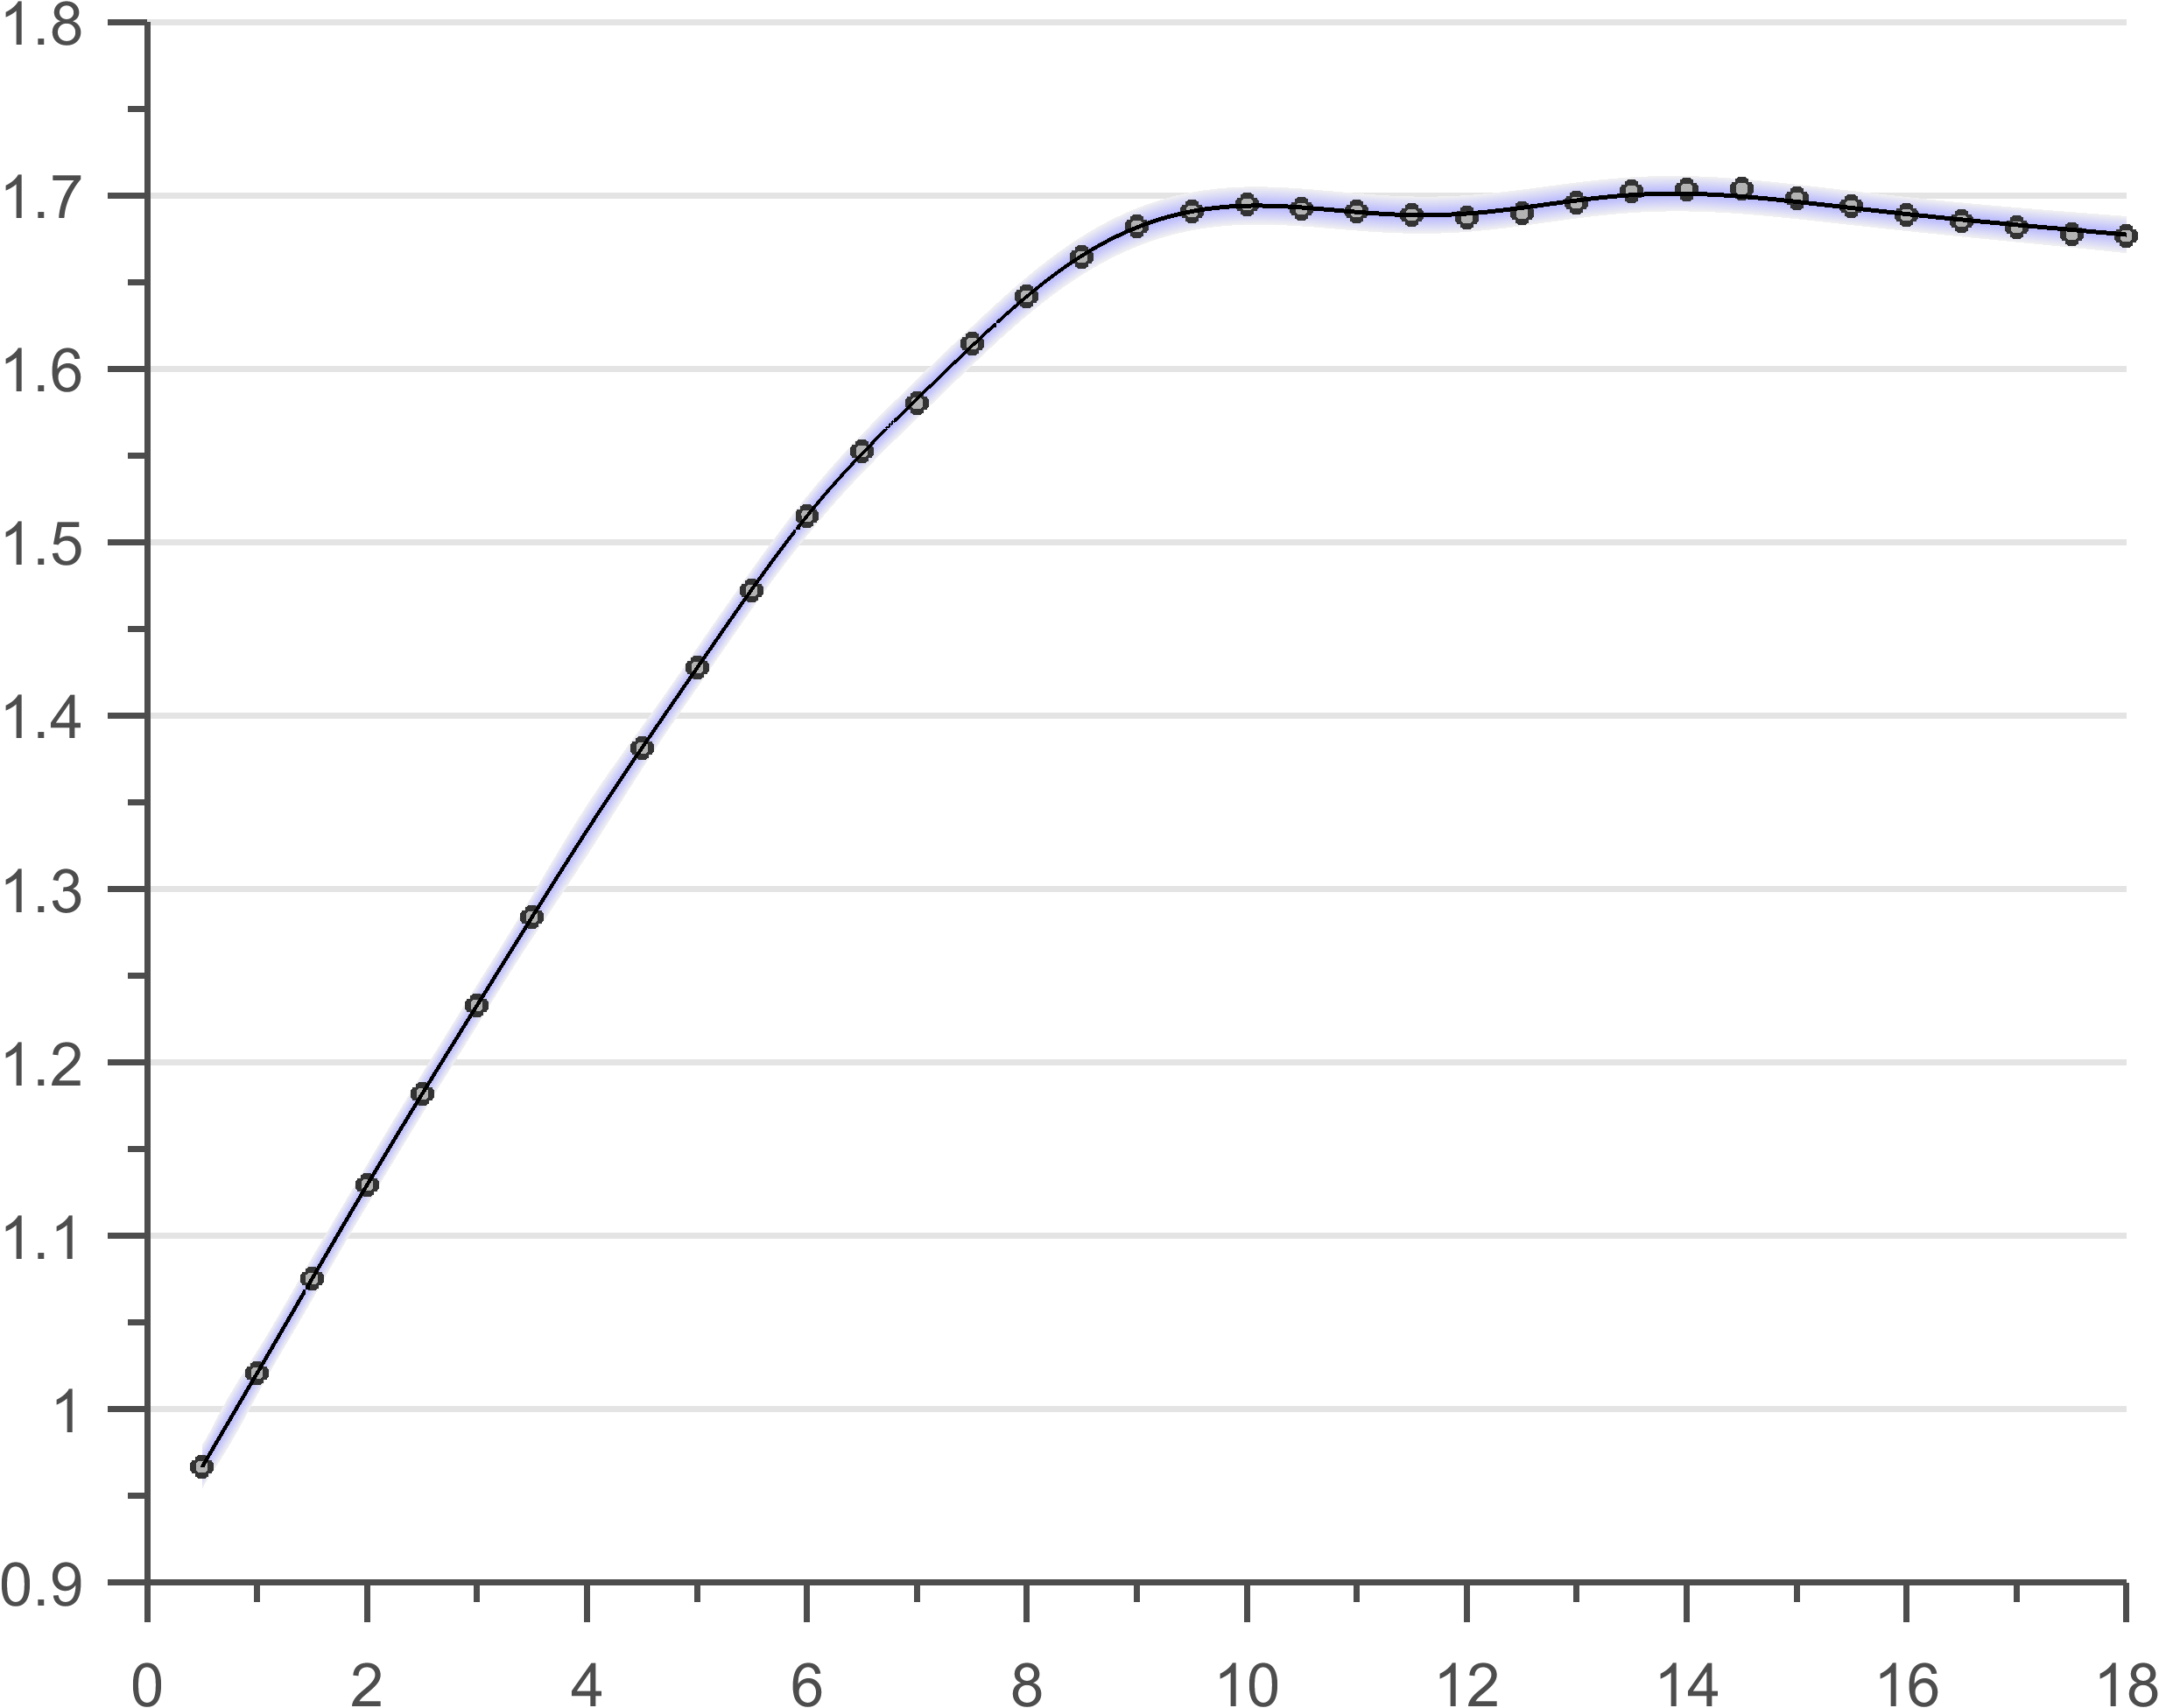
\includegraphics[width=0.45\textwidth]{images/clAlphaCovSE}
	    \label{subfig:clAlphaCovSE}}
	    \quad
    \subfigure[GP regression using a CP(linear, SE) kernel]
	    {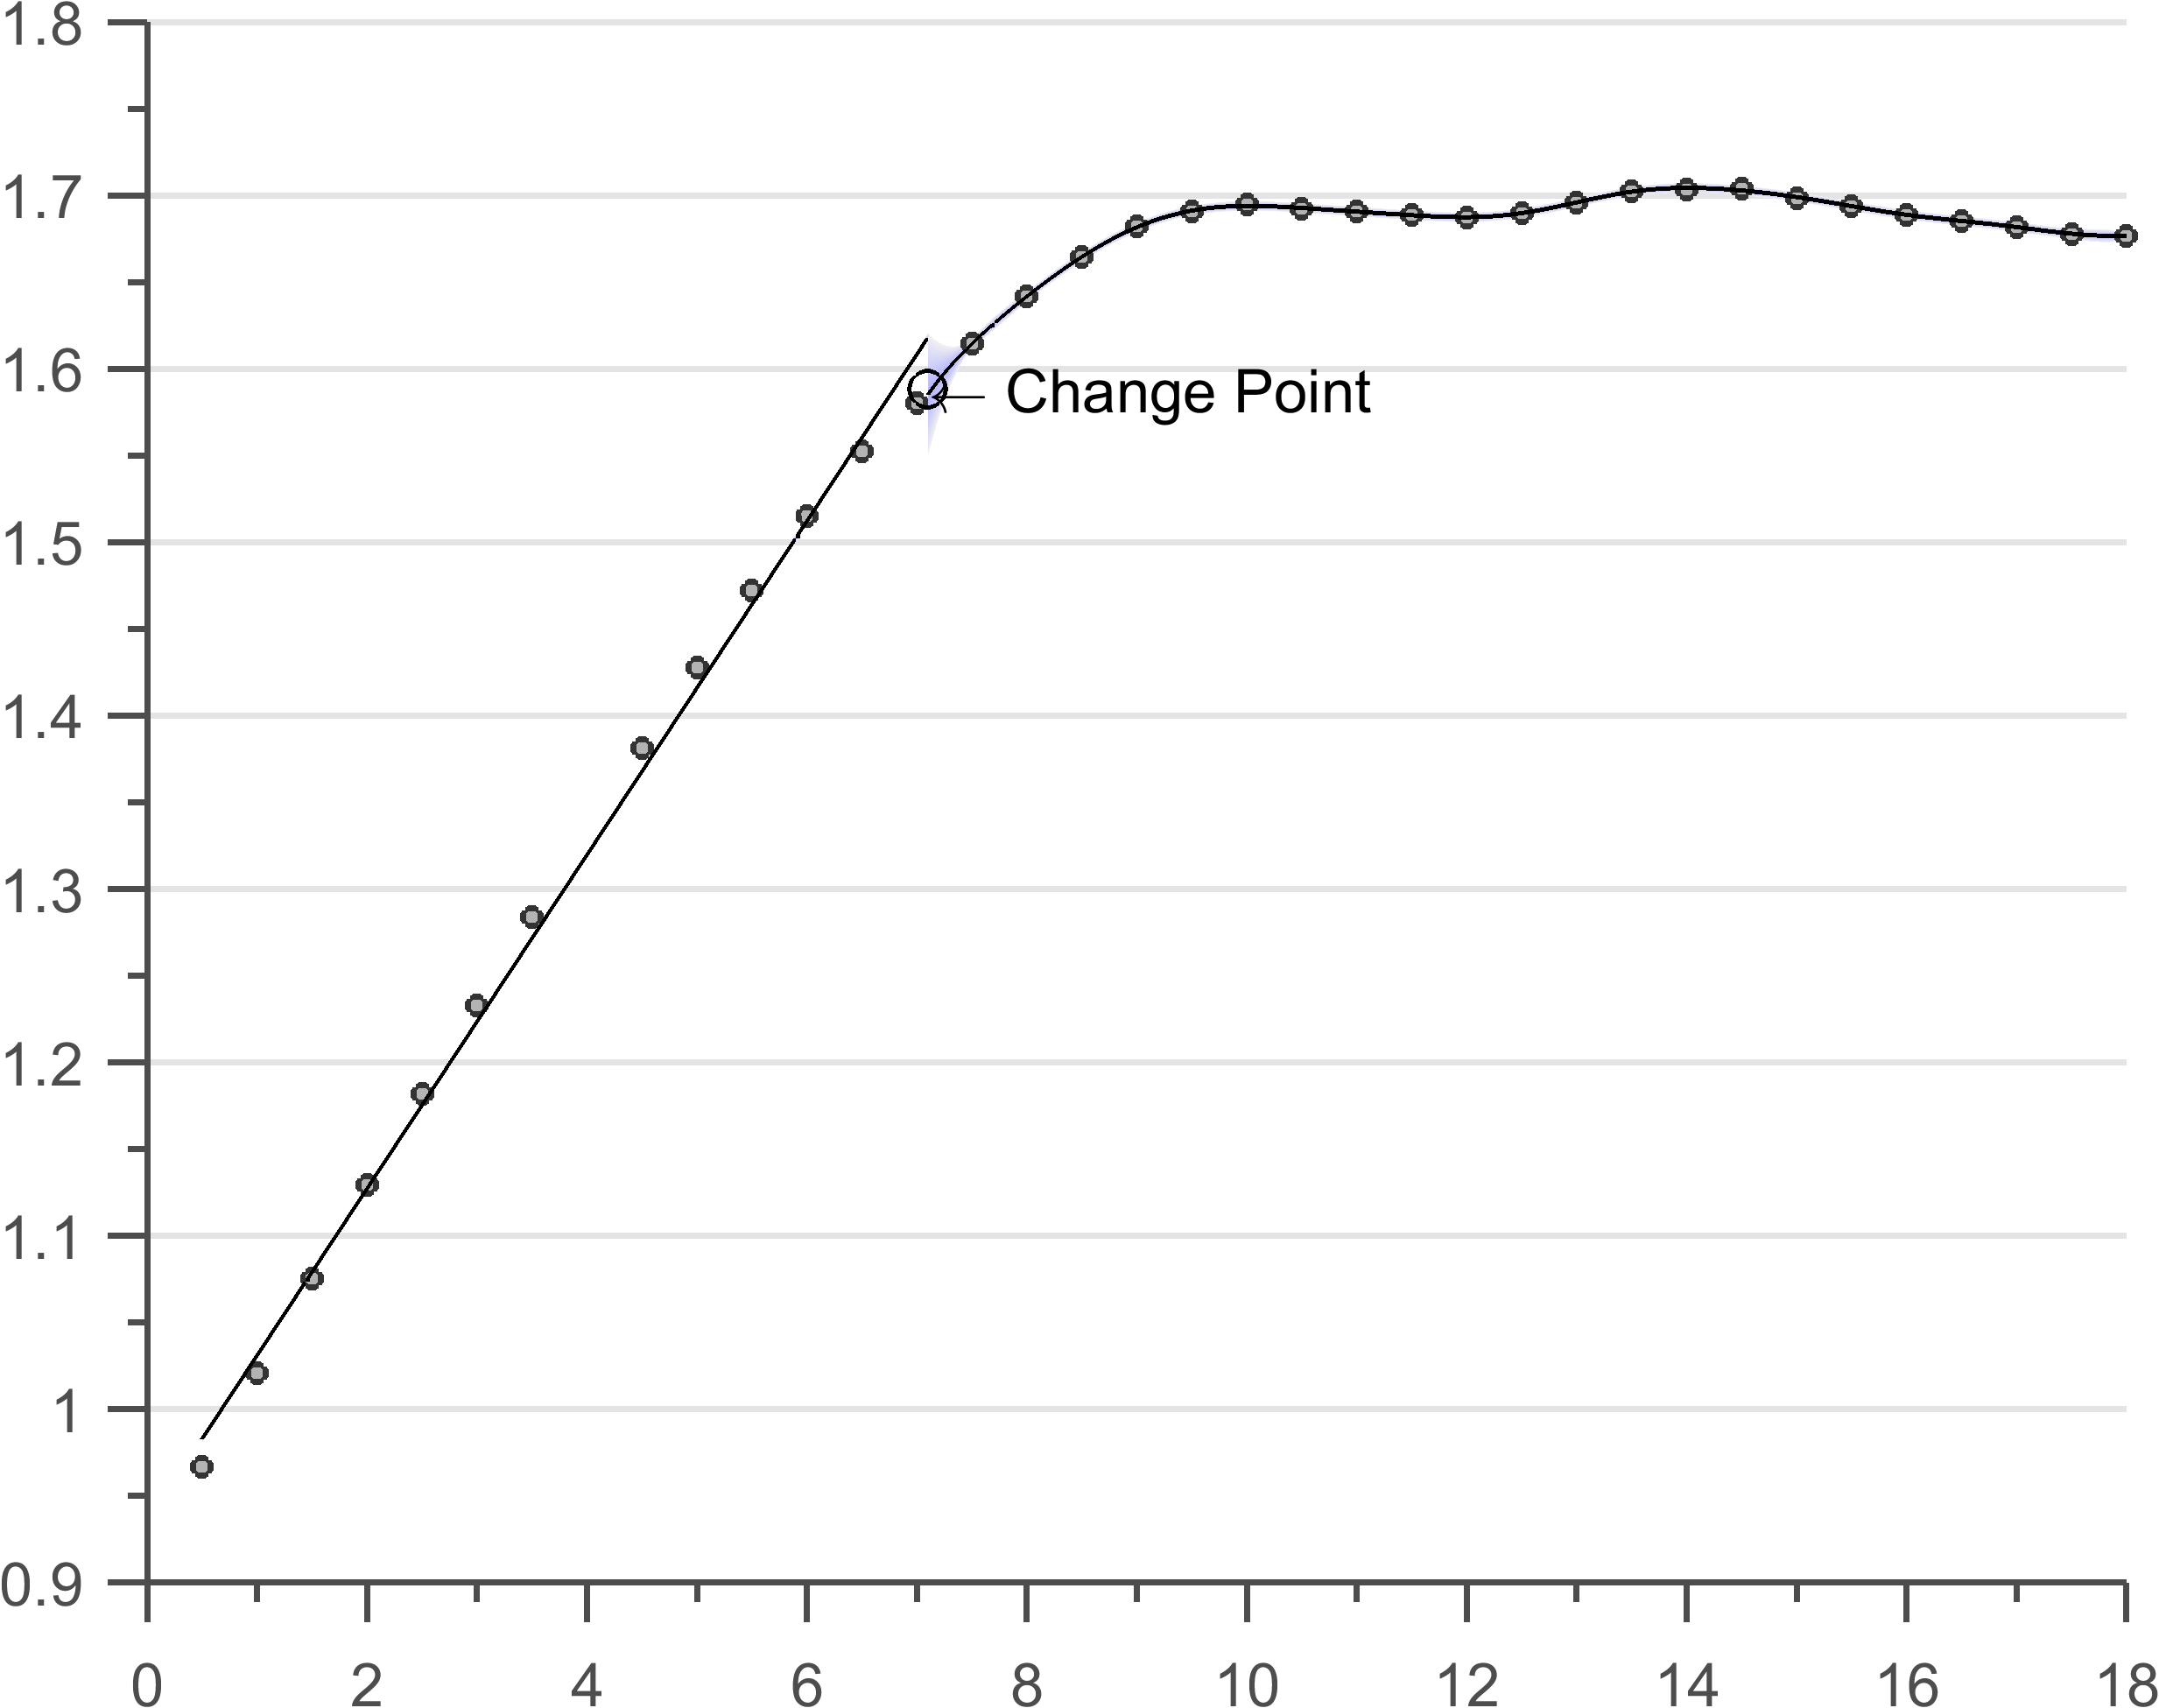
\includegraphics[width=0.45\textwidth]{images/clAlphaCovCP}
	    \label{subfig:clAlphaCovCP}}
	    \caption{Estimation of lift coefficient $Cl\alpha$}
\end{figure}


We tried to solve the problem of estimating the lift coefficient using Gaussian Process. Using the changepoint kernel which transitions from linear domain (linear kernel) to non-linear domain (SE kernel), prior assumptions of the problem were encoded in the kernel structure. Open source data for the lift vs alpha curves for the NACA 0012 airfoil were chosen. Fig: \ref{subfig:clAlphaCovSE} shows the regression of the data using SE kernel. Fig: \ref{subfig:clAlphaCovCP} regression of the same dataset using the CP(linear, SE) kernel. 

We can observe that the algorithm predicts a changepoint for the dataset. This is the point with where the linear assumptions start failing, according to prior information. The marginal likelihood of CP(linear, SE) kernel is rigged with many local minimas. The algorithm tries to put a changepoint at every observation point. Hence using a global optimizer is advised. The changepoint kernel is also very numerically unstable hence cross-validating the learners is also very important (model ensembles \ref{subsec:modelEnsembles}). The results of this study will be presented in the SIAM Uncertainty Quantification 2016 Conference.

\subsection{Spectral Mixture Kernel}
Spectral mixture kernels expand the hypothesis space by exploiting the Bochner's theorem \cite{bochner1959lectures}. It defines a scale-location mixture of finite Gaussian's in the frequency domain \cite{wilson2013gaussian}. 

\begin{align}
k_{\textrm{SM}}(x, x') = \sum_{q=1}^{Q}w_{q}cos(2\pi\mu_{q}^{T}\tau)\prod_{p=1}^{P}exp(-2\pi^{2}\tau_{p}^{2}\nu_{p})
\end{align}

In the frequency domain: the $\mu$ corresponds to modal frequencies; the $\nu$ correspond to damping values and the $w$ corresponds to amplitude or weights of individual gaussians. The Spectral Mixture kernel performs surprisingly well in pattern discovery and extrapolation tasks. But, it falls in the similar trade-off of bias vs variance \ref{subsec:biasVsVariance}. In our experiments the Spectral Mixture kernel performs significantly well in time-series tasks.

\subsubsection{Identifying structural modal parameters using Spectral Mixture Kernel}
Modal analysis has been widely used as a means of identifying dynamic properties such as modal frequencies, damping ratios and mode shapes of a structural system. Traditionally, the system is subjected to artificial input excitations and output deformations (displacements, velocities or accelerations) are measured. These later help in identifying the modal parameters of the system, this process is called Experimental Modal Analysis (EMA). 

Since the last decade Operational Modal Analysis (OMA) has gained considerable interest in the community. OMA identifies the modal parameters only from the output measurements while assuming ambient excitations as random noise. OMA is cheaper because it does not require expensive experimental setup and and can be used in real time operational use cases such as health monitoring \cite{peeters2005industrial} \cite{shahdin2010correlating} \cite{rainieri2007automated}. Several algorithms in OMA can be seen as extensions of EMA algorithms based on the similar assumption of second order MDOF system.

\begin{figure*}[!ht]
  \centering
  \subfigure[Measured output on accelerometers \(x(t)\)]
  {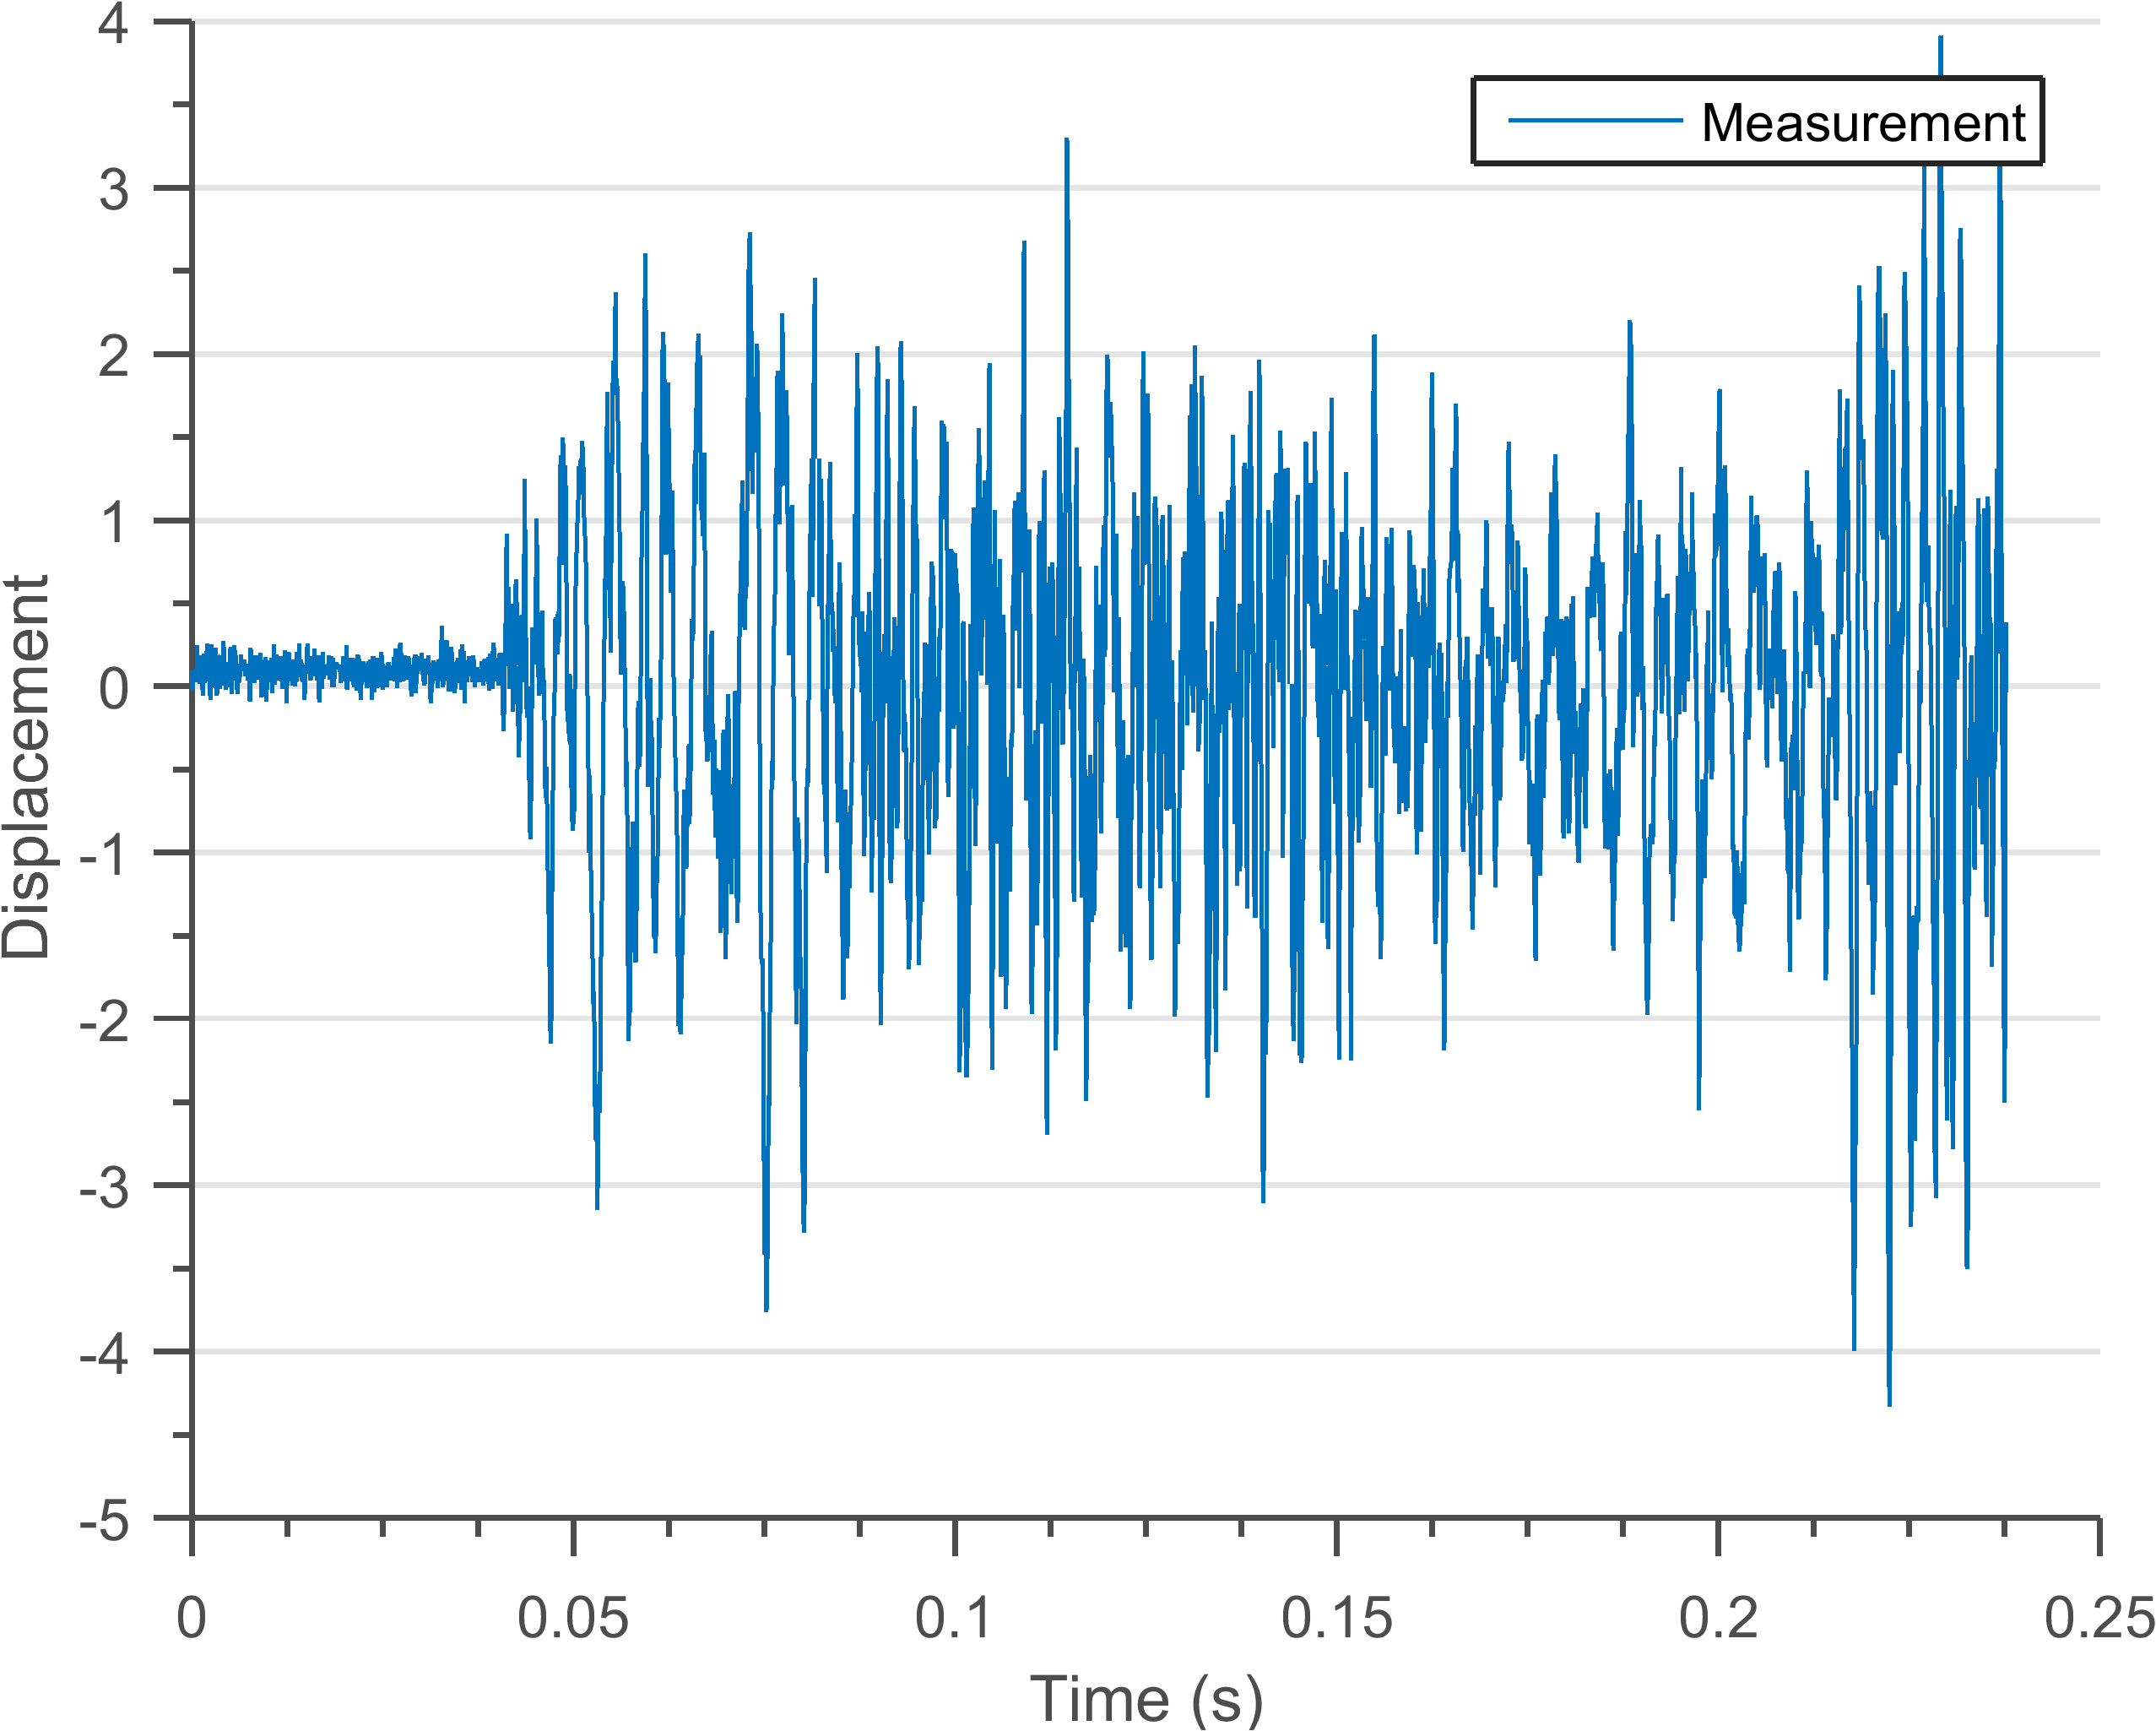
\includegraphics[width=0.3\textwidth]{images/randomOutput}\label{subfig:randomOutput}}\quad
  \subfigure[Auto-correlation \(k(\tau)\) of the measured output fig: \ref{subfig:randomOutput}]
  {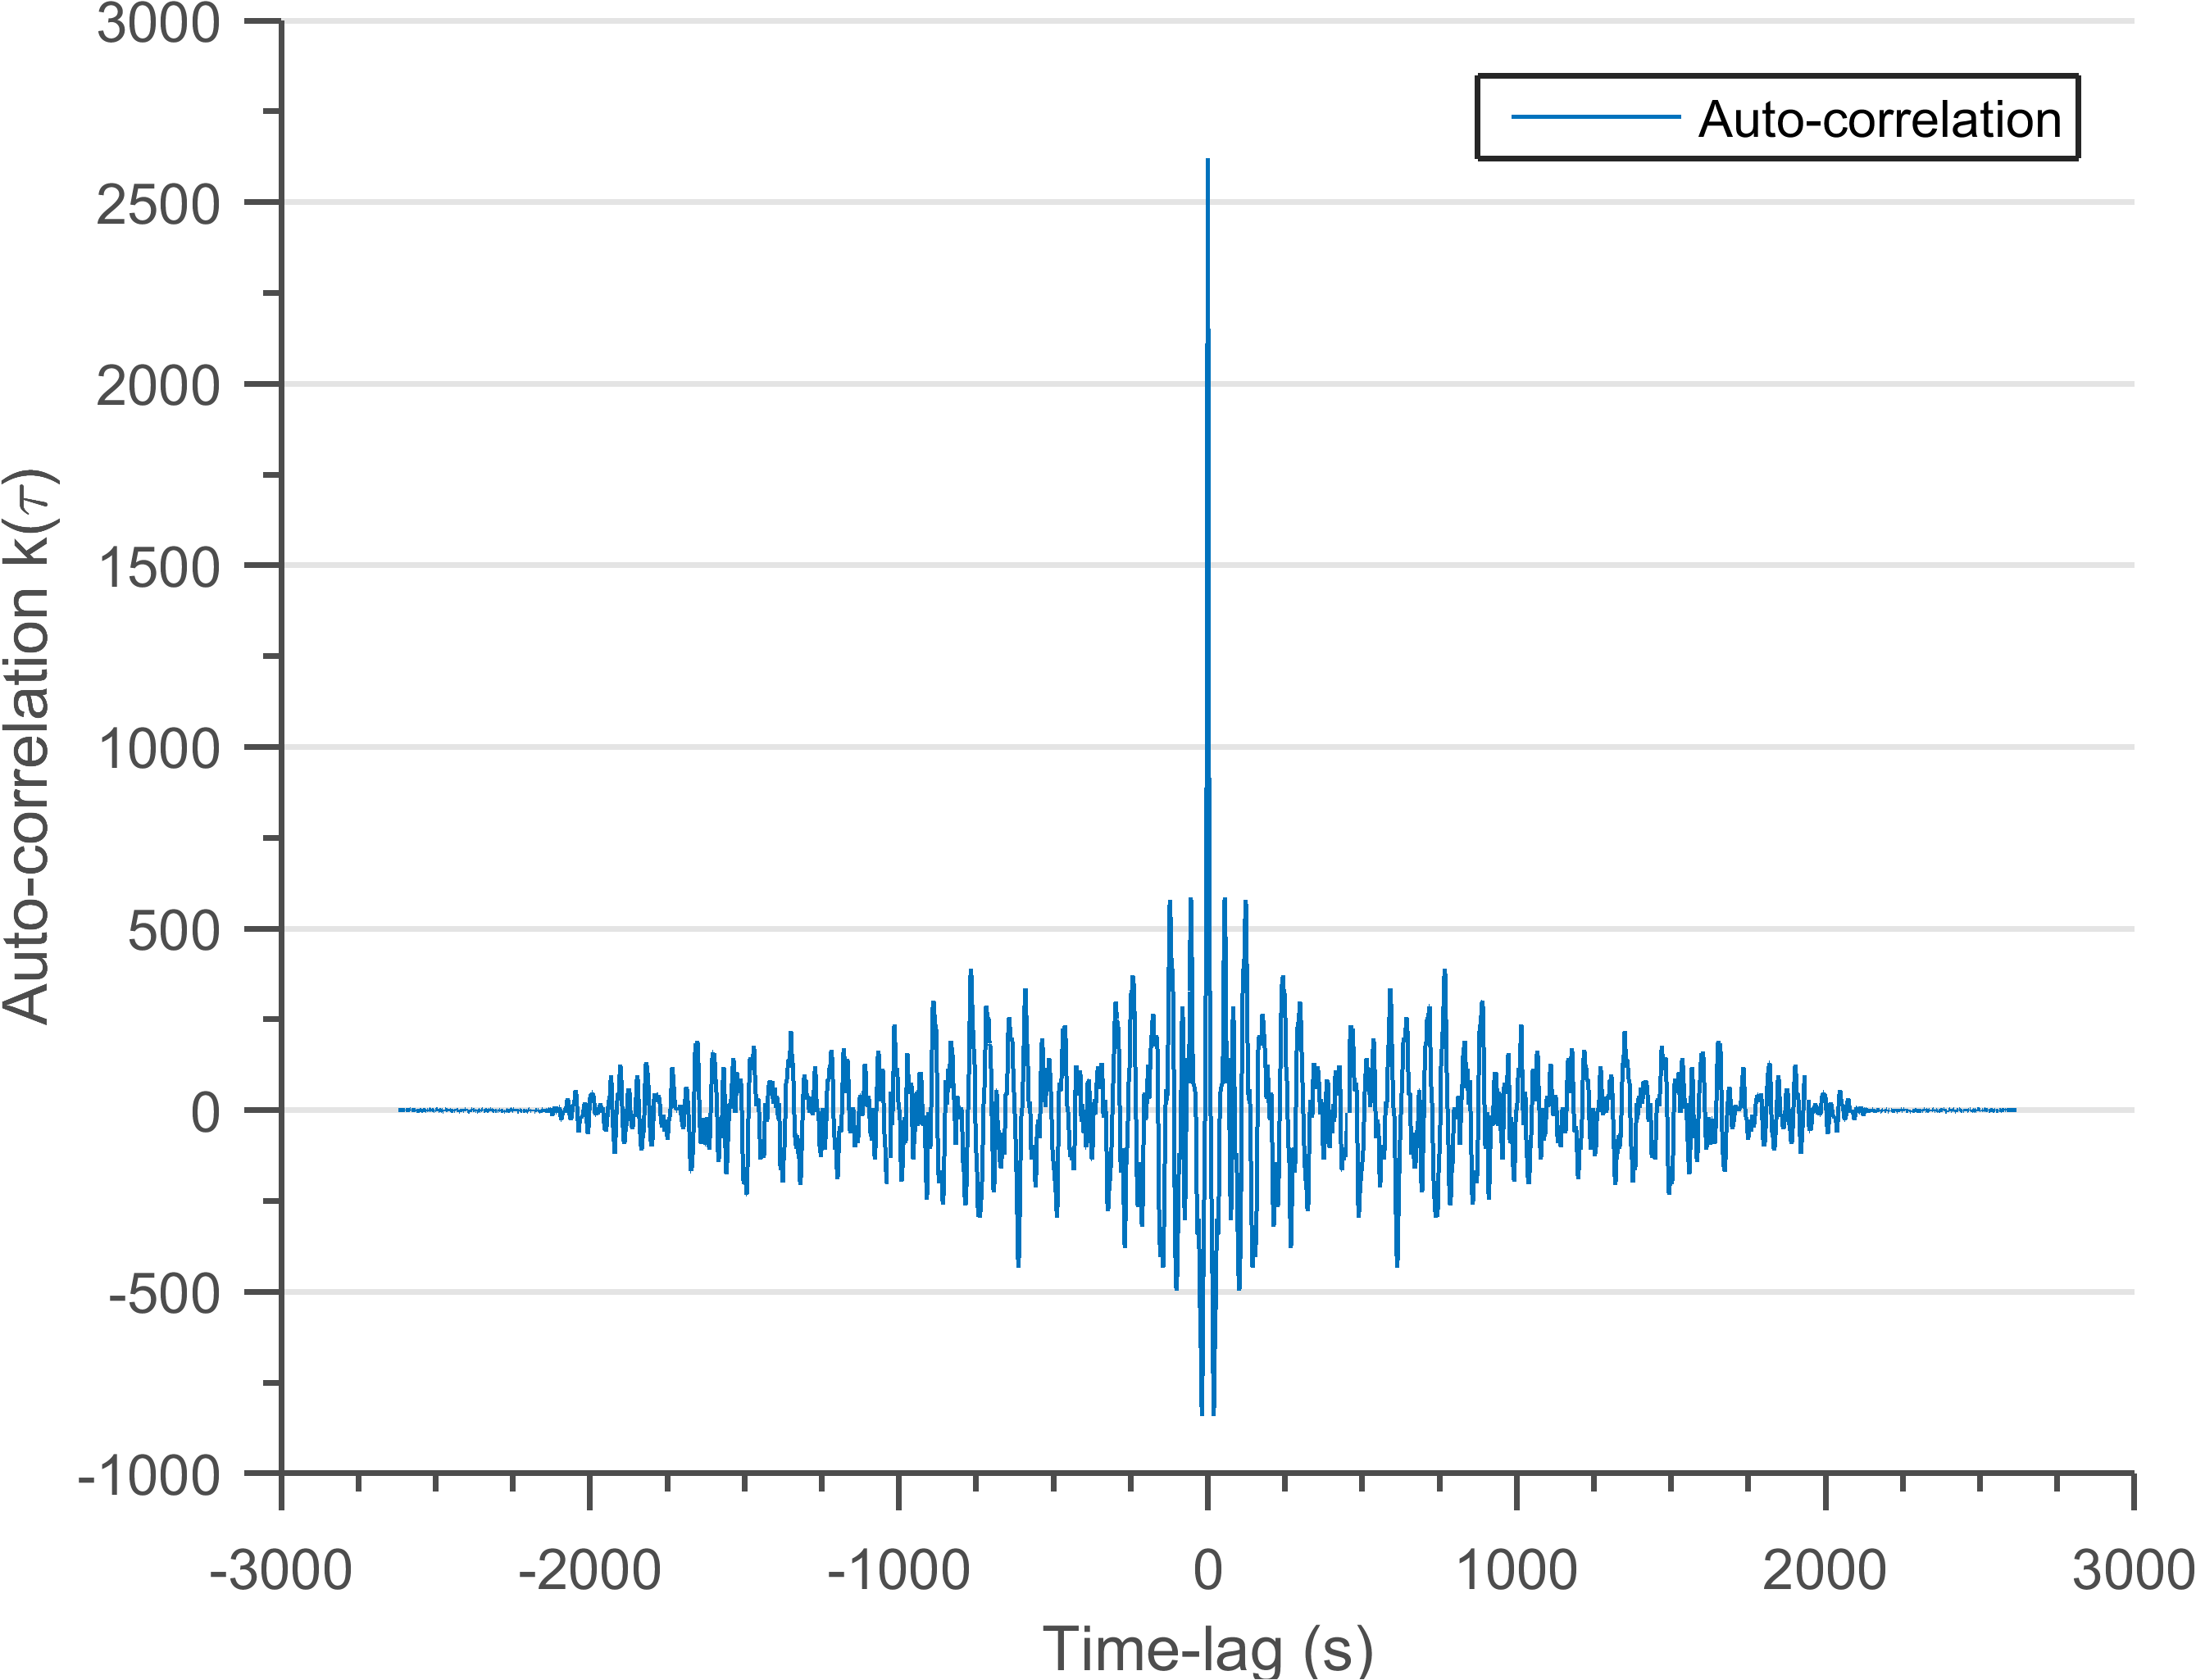
\includegraphics[width=0.3\textwidth]{images/autocorrelationOutput}\label{subfig:autocorrelationOutput}}\quad
  \subfigure[Power spectrum density \(S(s)\) of the output fig: \ref{subfig:randomOutput}]
  {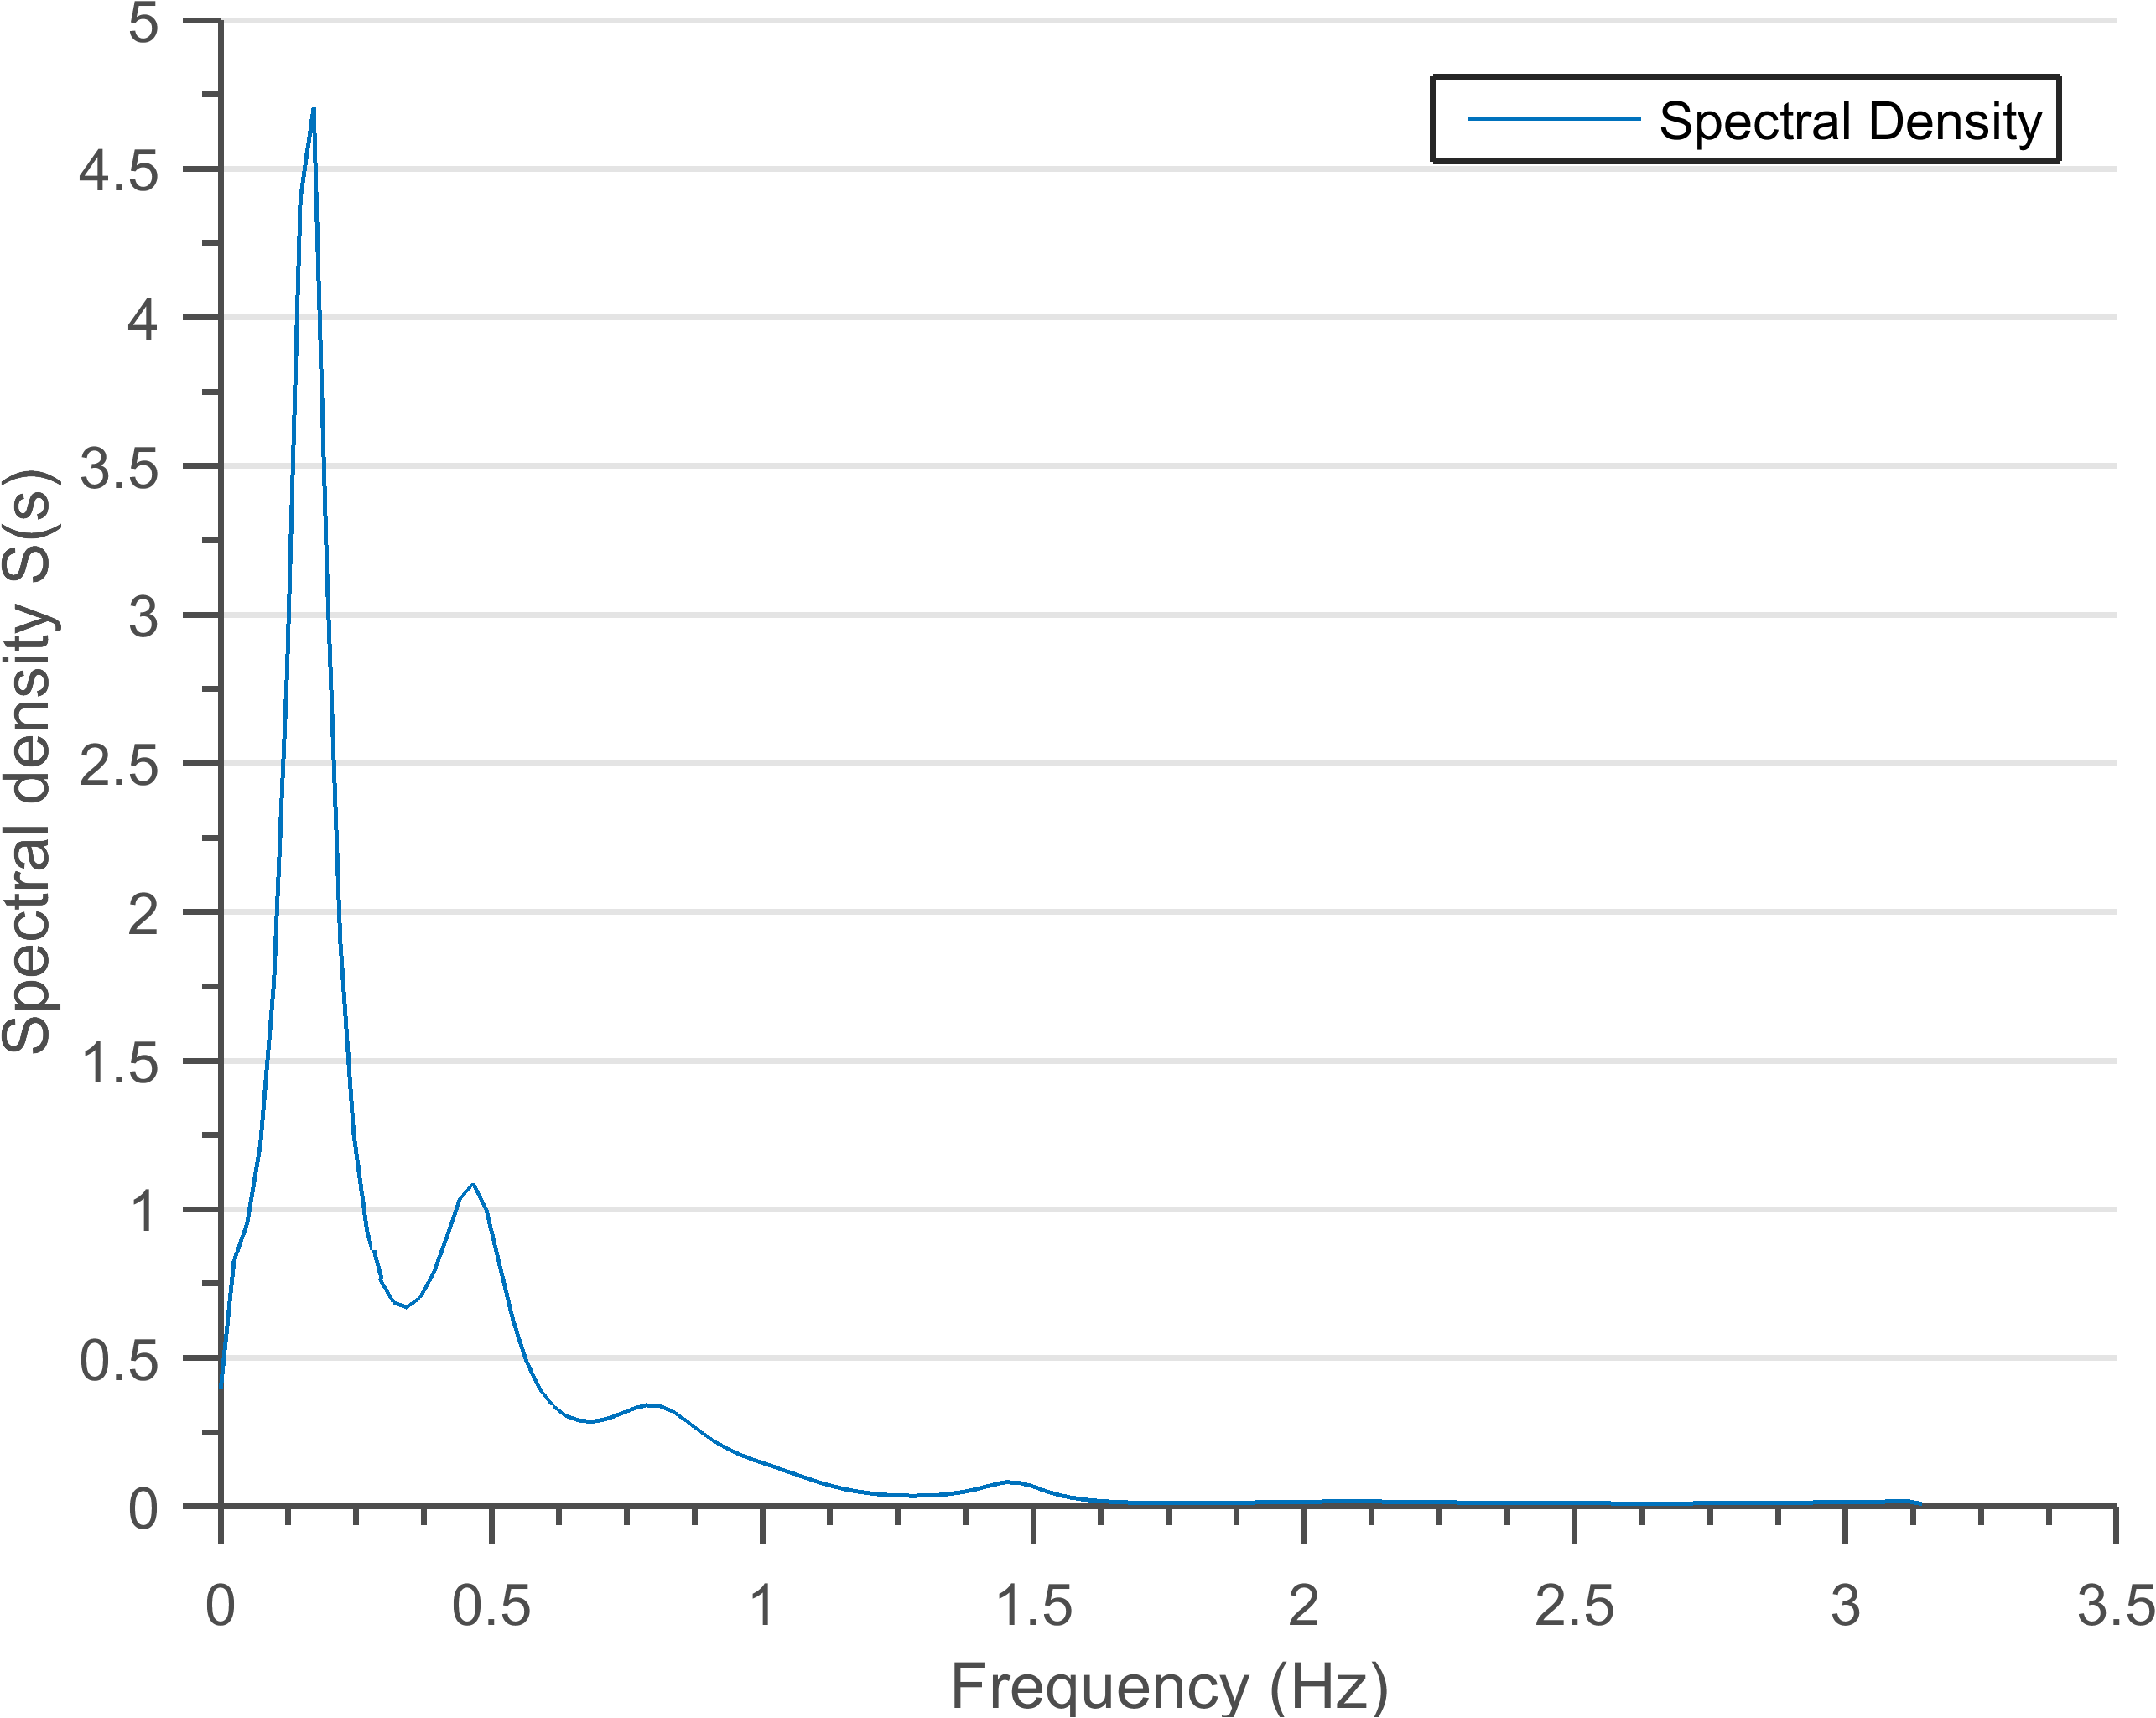
\includegraphics[width=0.3\textwidth]{images/psdOutput}\label{subfig:psdOutput}}
  
  \caption{Different types of measurements for estimation of Modal parameters in OMA}
\end{figure*}

\indent If we assume the measurement \(x(t)\) to be a stationary random process, then according to bochner's theorem \cite{bochner2016lectures} the spectral density or power spectrum \(S(s)\) can be represented as equation \ref{eq:spectralDensity}.

\begin{equation}\label{eq:spectralDensity}
    S(s) = \int k(\tau)exp(-2 \pi i s^{T} \tau )d\tau 
\end{equation}
Here, \(S(s)\) is the power spectrum for the measurement \(x(t)\), where \(s\) lies in the frequency-damping plane. Figure \ref{subfig:psdOutput} shows the power spectrum calculated for the measurement \(x(t)\) shown in figure \ref{subfig:randomOutput}. 

Initially the Peak Picking technique (PP) \cite{gade2005frequency} was used in the frequency-domain to identify modal frequencies and shapes. The PP technique is a very easy way to identify modes but becomes inefficient for complex structures \cite{zhang2004overview}. This gave rise to the Frequency Domain Decomposition (FDD) \cite{brincker2000modal} where modal frequency are denoted as the eigenvalues of spectral density matrix equation \ref{eq:FDD}.

Majority of frequency-domain algorithms in EMA fit a Rational Fractional Polynomial (RFP) \cite{richardson1982parameter} in the frequency domain for modal identification \cite{allemang1998unified} \cite{chauhan2007unified}. The Rational Fractional Polynomial equation \ref{eq:RFP} form can be derived if we assume the system to be second order differential equation \ref{eq:secondOrderSystem}.
\begin{table*}[t]
  \centering
  \setlength\extrarowheight{8pt}
\begin{tabular}{ |c|c|c| } 
  \hline
  Measurement; eg. figure \ref{subfig:randomOutput} & Auto-correlation; eg. figure \ref{subfig:autocorrelationOutput} & Power Spectrum; eg. figure \ref{subfig:psdOutput} \\
  \hline
  $x(t)$ & $k(\tau) = \int x(t)x(t-\tau)dt$ &  $S(s) = \int k(\tau)exp(-2 \pi i s^{T} \tau )d\tau$\\
  \hline \hline
  \multicolumn{3}{|c|}{Assumption: Second Order Differential}\\
  \hline
   & $k(\tau) = \sum A_{i}exp(-\lambda_{i}\tau)sin(B_{i}\tau)$ & $S(j\omega) = \frac{\sum a_{k}(j\omega)^{k}}{\sum b_{l}(j\omega)^{l}}$\\
   \hline \hline
   \multicolumn{3}{|c|}{Assumption: Gaussian Mixture Model}\\
   \hline
   $x(t) = GP(0 , cov_{SM})$ 
   & $k(\tau) = \sum w_{i} cos(2\pi\mu_{i}\tau) exp\{-2\pi^{2}\sigma_{i}^{2}\tau^{2}\}$ 
   & $S(s) = \sum w_{i}  \frac{1}{\sqrt{2\pi\sigma_{i}^{2}}}exp\{\frac{1}{2\sigma_{i}^{2}}(s-\mu_{i})^{2}\} $\\
   \hline
\end{tabular}
  \caption{Comparison of fitting functions}
  \label{tab:comparisonOfFittingFunctions}
\end{table*}

Moreover, if we assume that \(x(t)\) is a zero-mean gaussian process, then we can transform GMM in frequency-domain to time-domain. The equation \ref{eq:GMM} and equation \ref{eq:timeDomainGMM} are equivalent to fitting a zero-mean gaussian process with a spectral mixture covariance function \cite{wilson2013gaussian}.

\begin{equation}\label{eq:dataDomainGMM}
    x(t) = GP(0 , cov_{SM}(t, t'))
\end{equation}

Here, \(GP\) denotes a gaussian process \cite{Rasmussen2005}, while \(cov_{SM}\) represents a spectral mixture covariance function which resembles equation \ref{eq:timeDomainGMM} \cite{wilson2013gaussian}. 

We would like to emphasize that keeping the computational complexities aside, fitting a spectral mixture gaussian process in time-domain equation \ref{eq:GMM}, fitting equation \ref{eq:timeDomainGMM} for covariance-driven modal identification and fitting a GMM equation \ref{eq:GMM} in the frequency-domain are equivalent. In fact the initial idea of this paper was to fit a Gaussian Process (GP) in the data domain, but GP's are computationally heavy and we achieved a good accuracy by fitting the GMM in frequency domain. Refer to table \ref{tab:comparisonOfFittingFunctions} for a more comprehensive view at various fitting functions.

\begin{figure*}[!ht]
  \centering
  \subfigure[Stabilization diagram with increasing number of gaussians $Q$, the dots denote the stabilized frequencies. We can observe that as the number of $Q$ increases the algorithm starts finding better and better modes.]
  {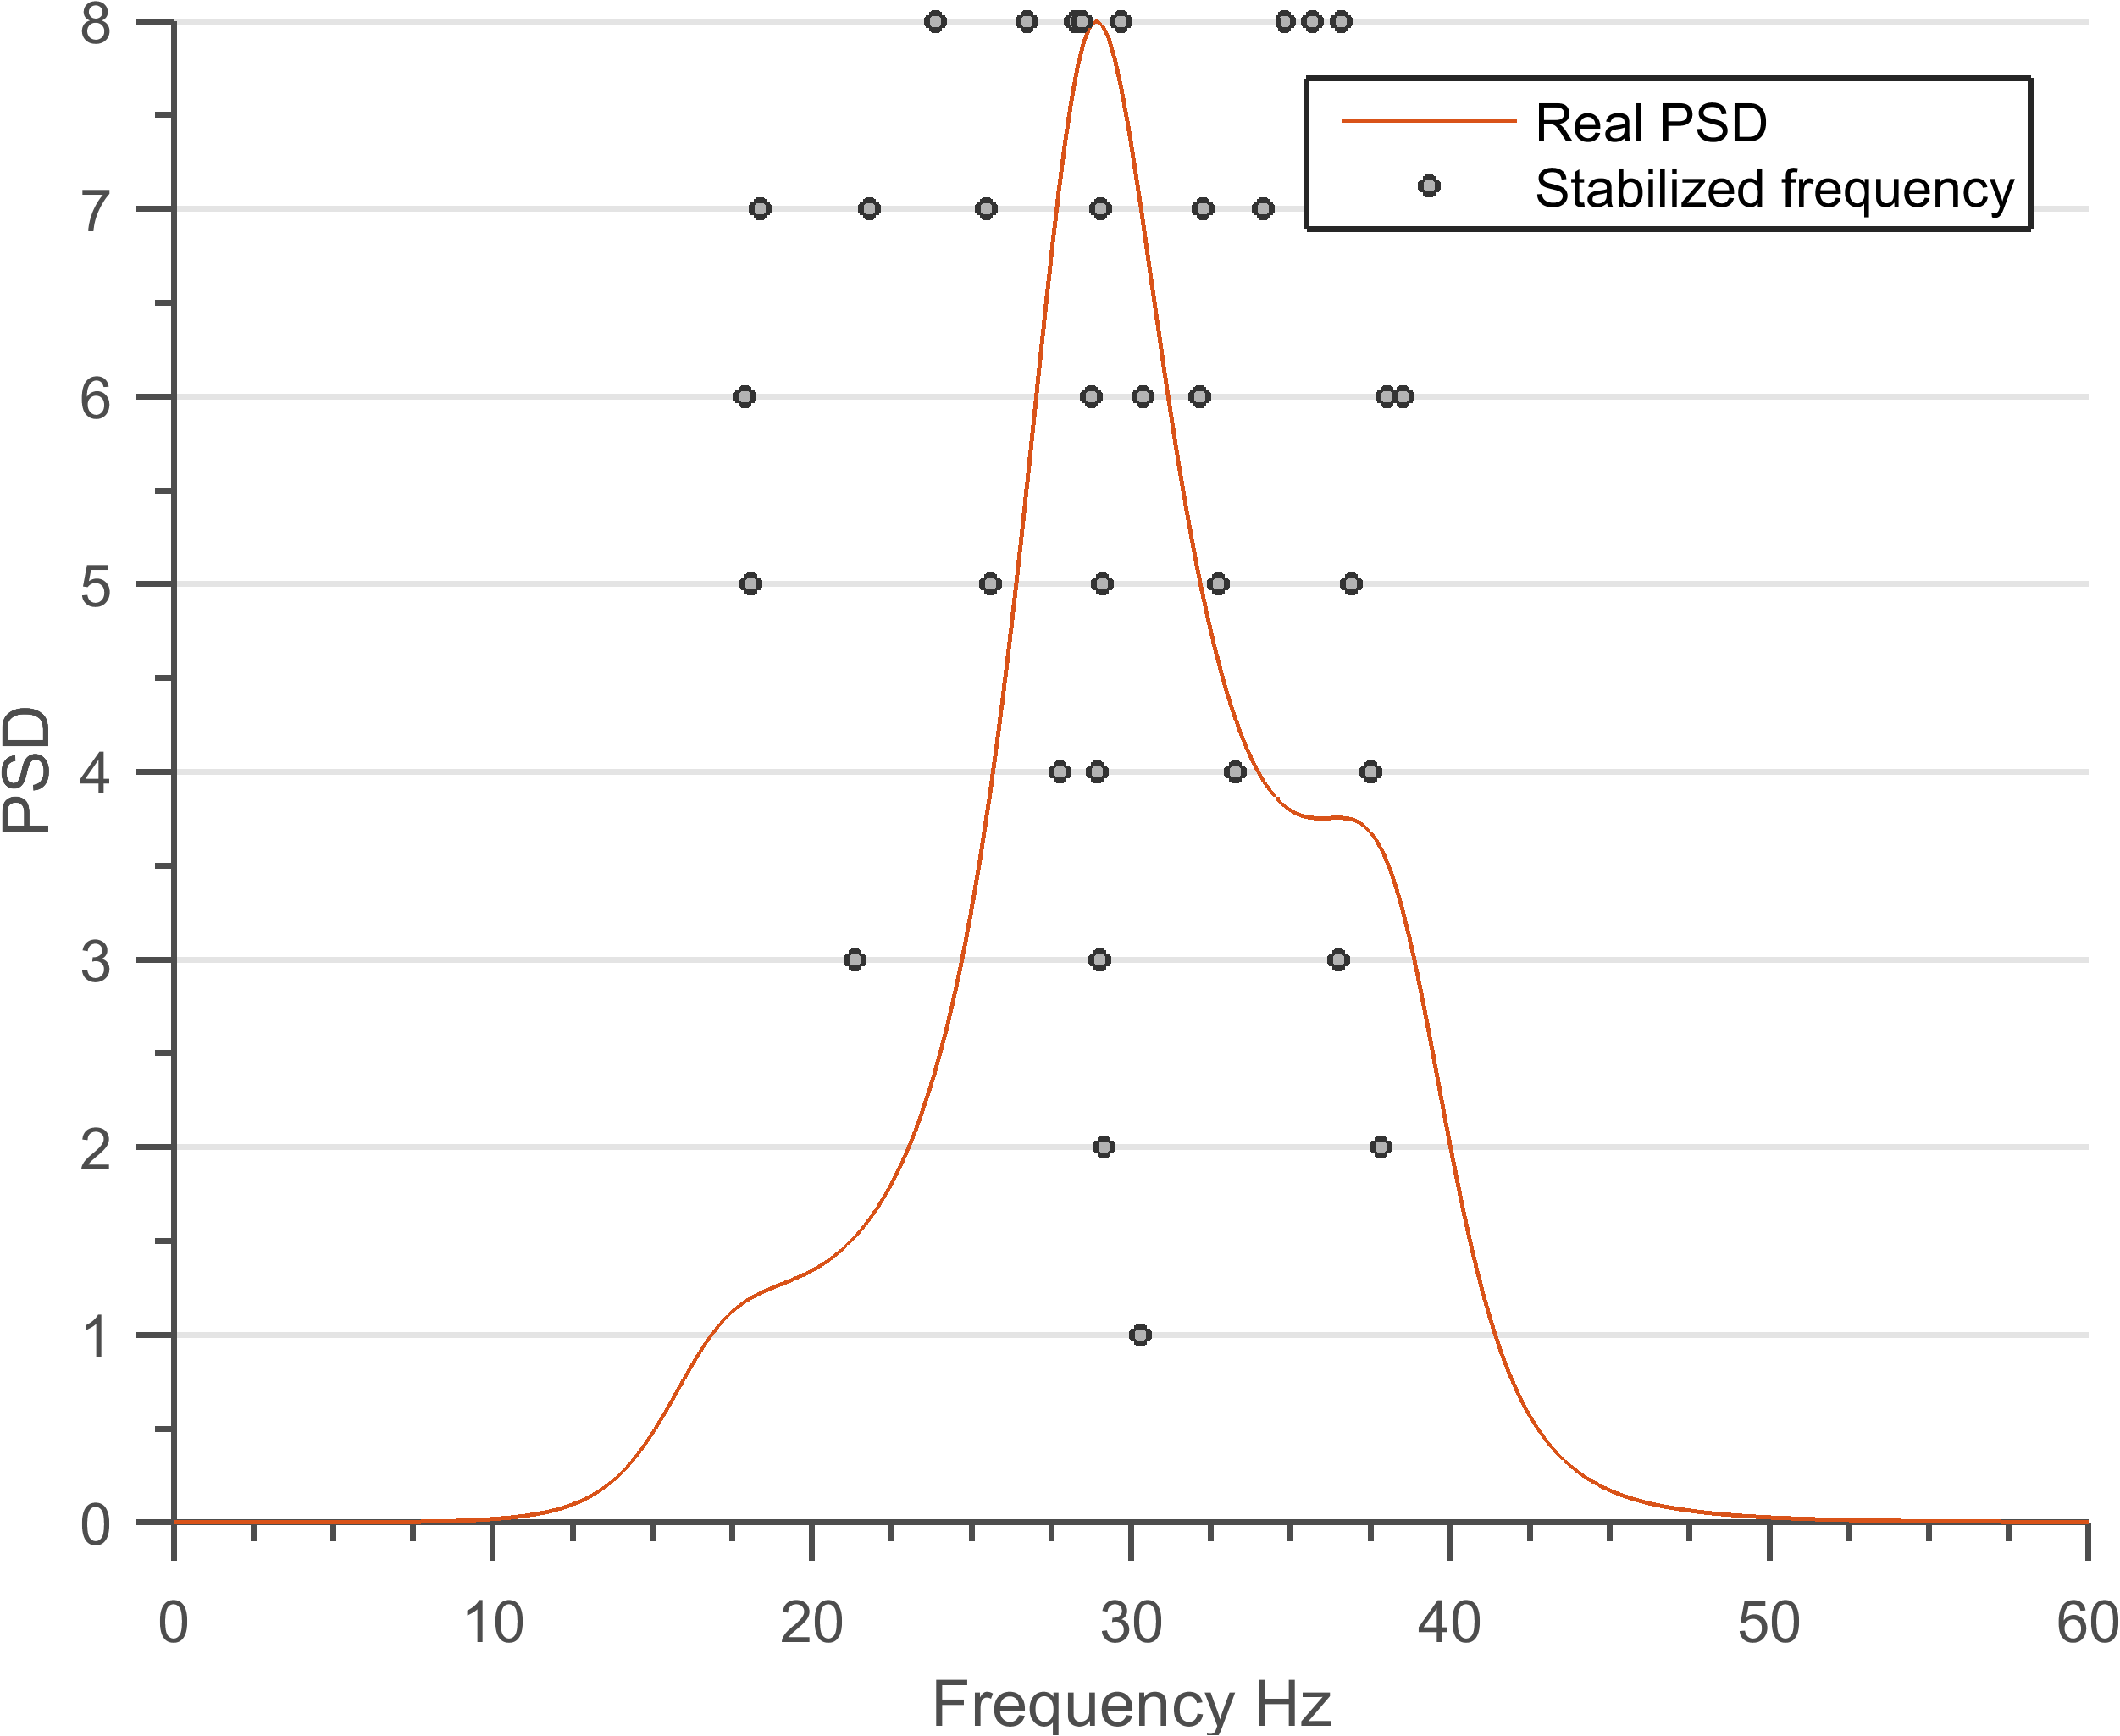
\includegraphics[width=0.3\textwidth]{images/stabilizationDiagram}\label{subfig:stabilizationDiagram}}\quad
    \subfigure[The BIC criterion with increasing number of gaussian's $Q$. We can see that that the BIC is minimum for $Q=6$ and hence if we add anymore gaussian's for our dataset we will be performing over-fitting]
  {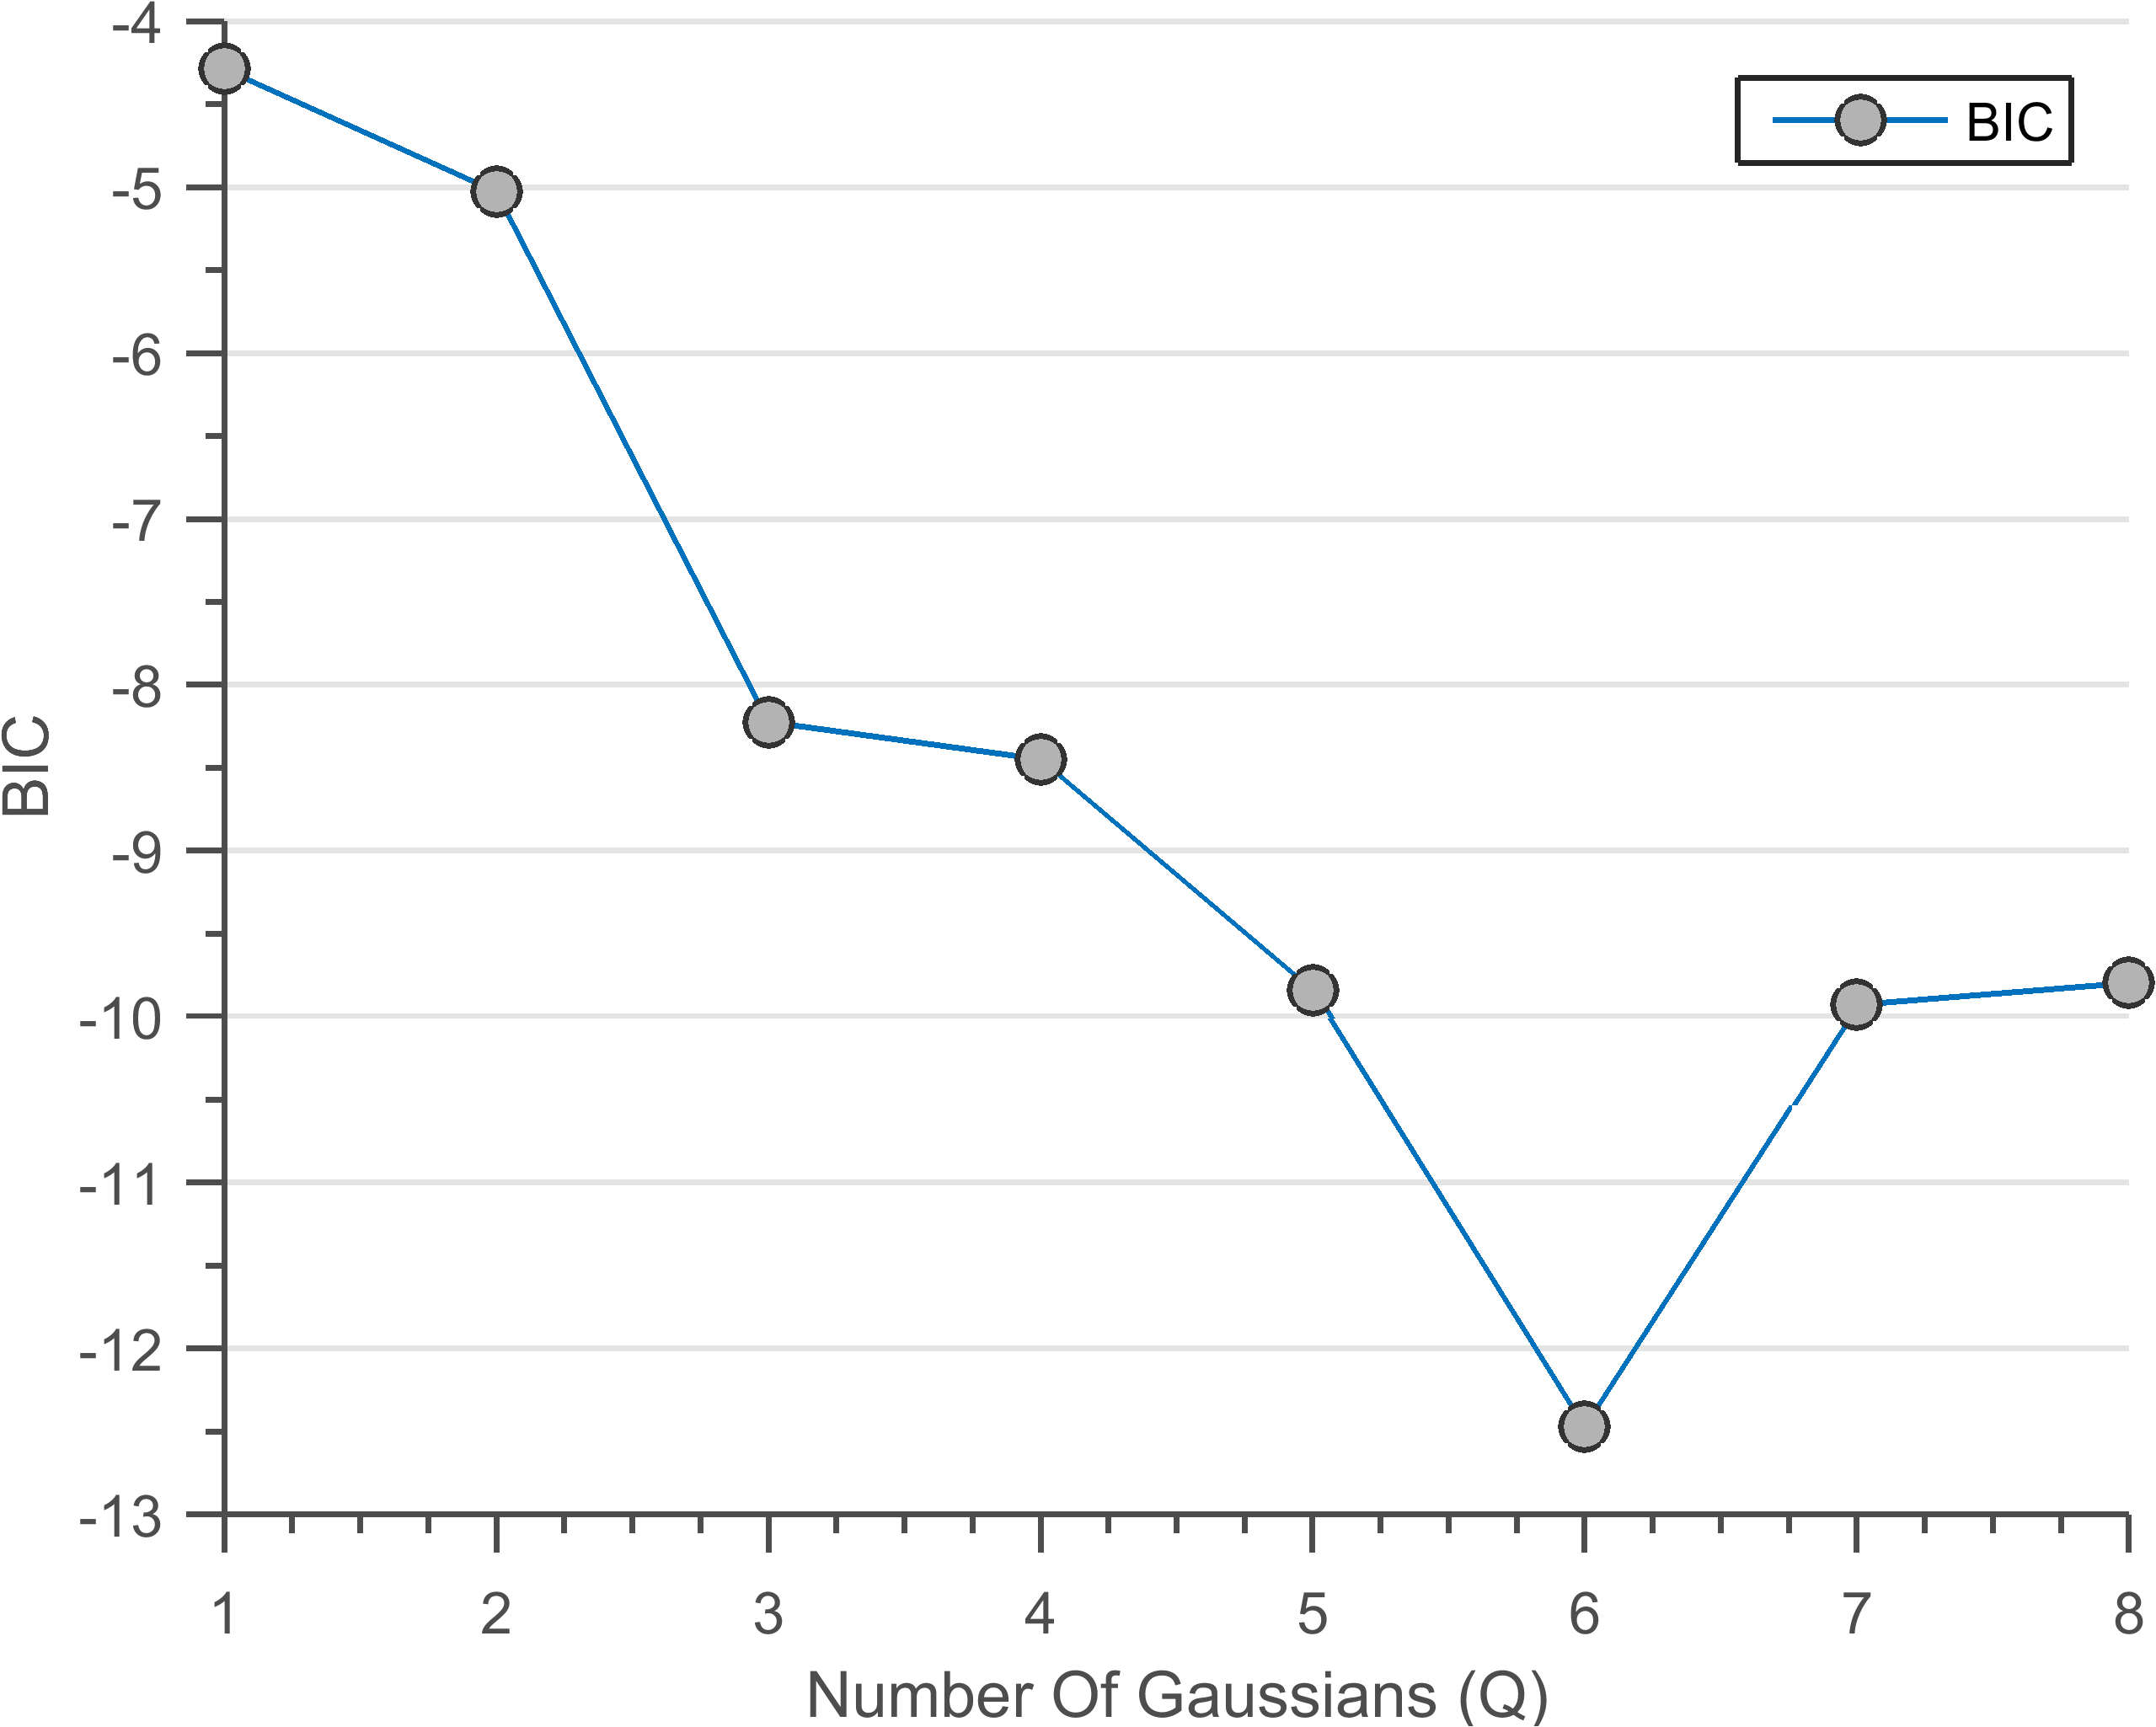
\includegraphics[width=0.3\textwidth]{images/bicVsQ}\label{subfig:bicVsQ}}\quad
  \subfigure[Distribution of  gaussians for $Q=6$. We can see that the three modal frequencies have majority of the participation in representing the spectral density.]
  {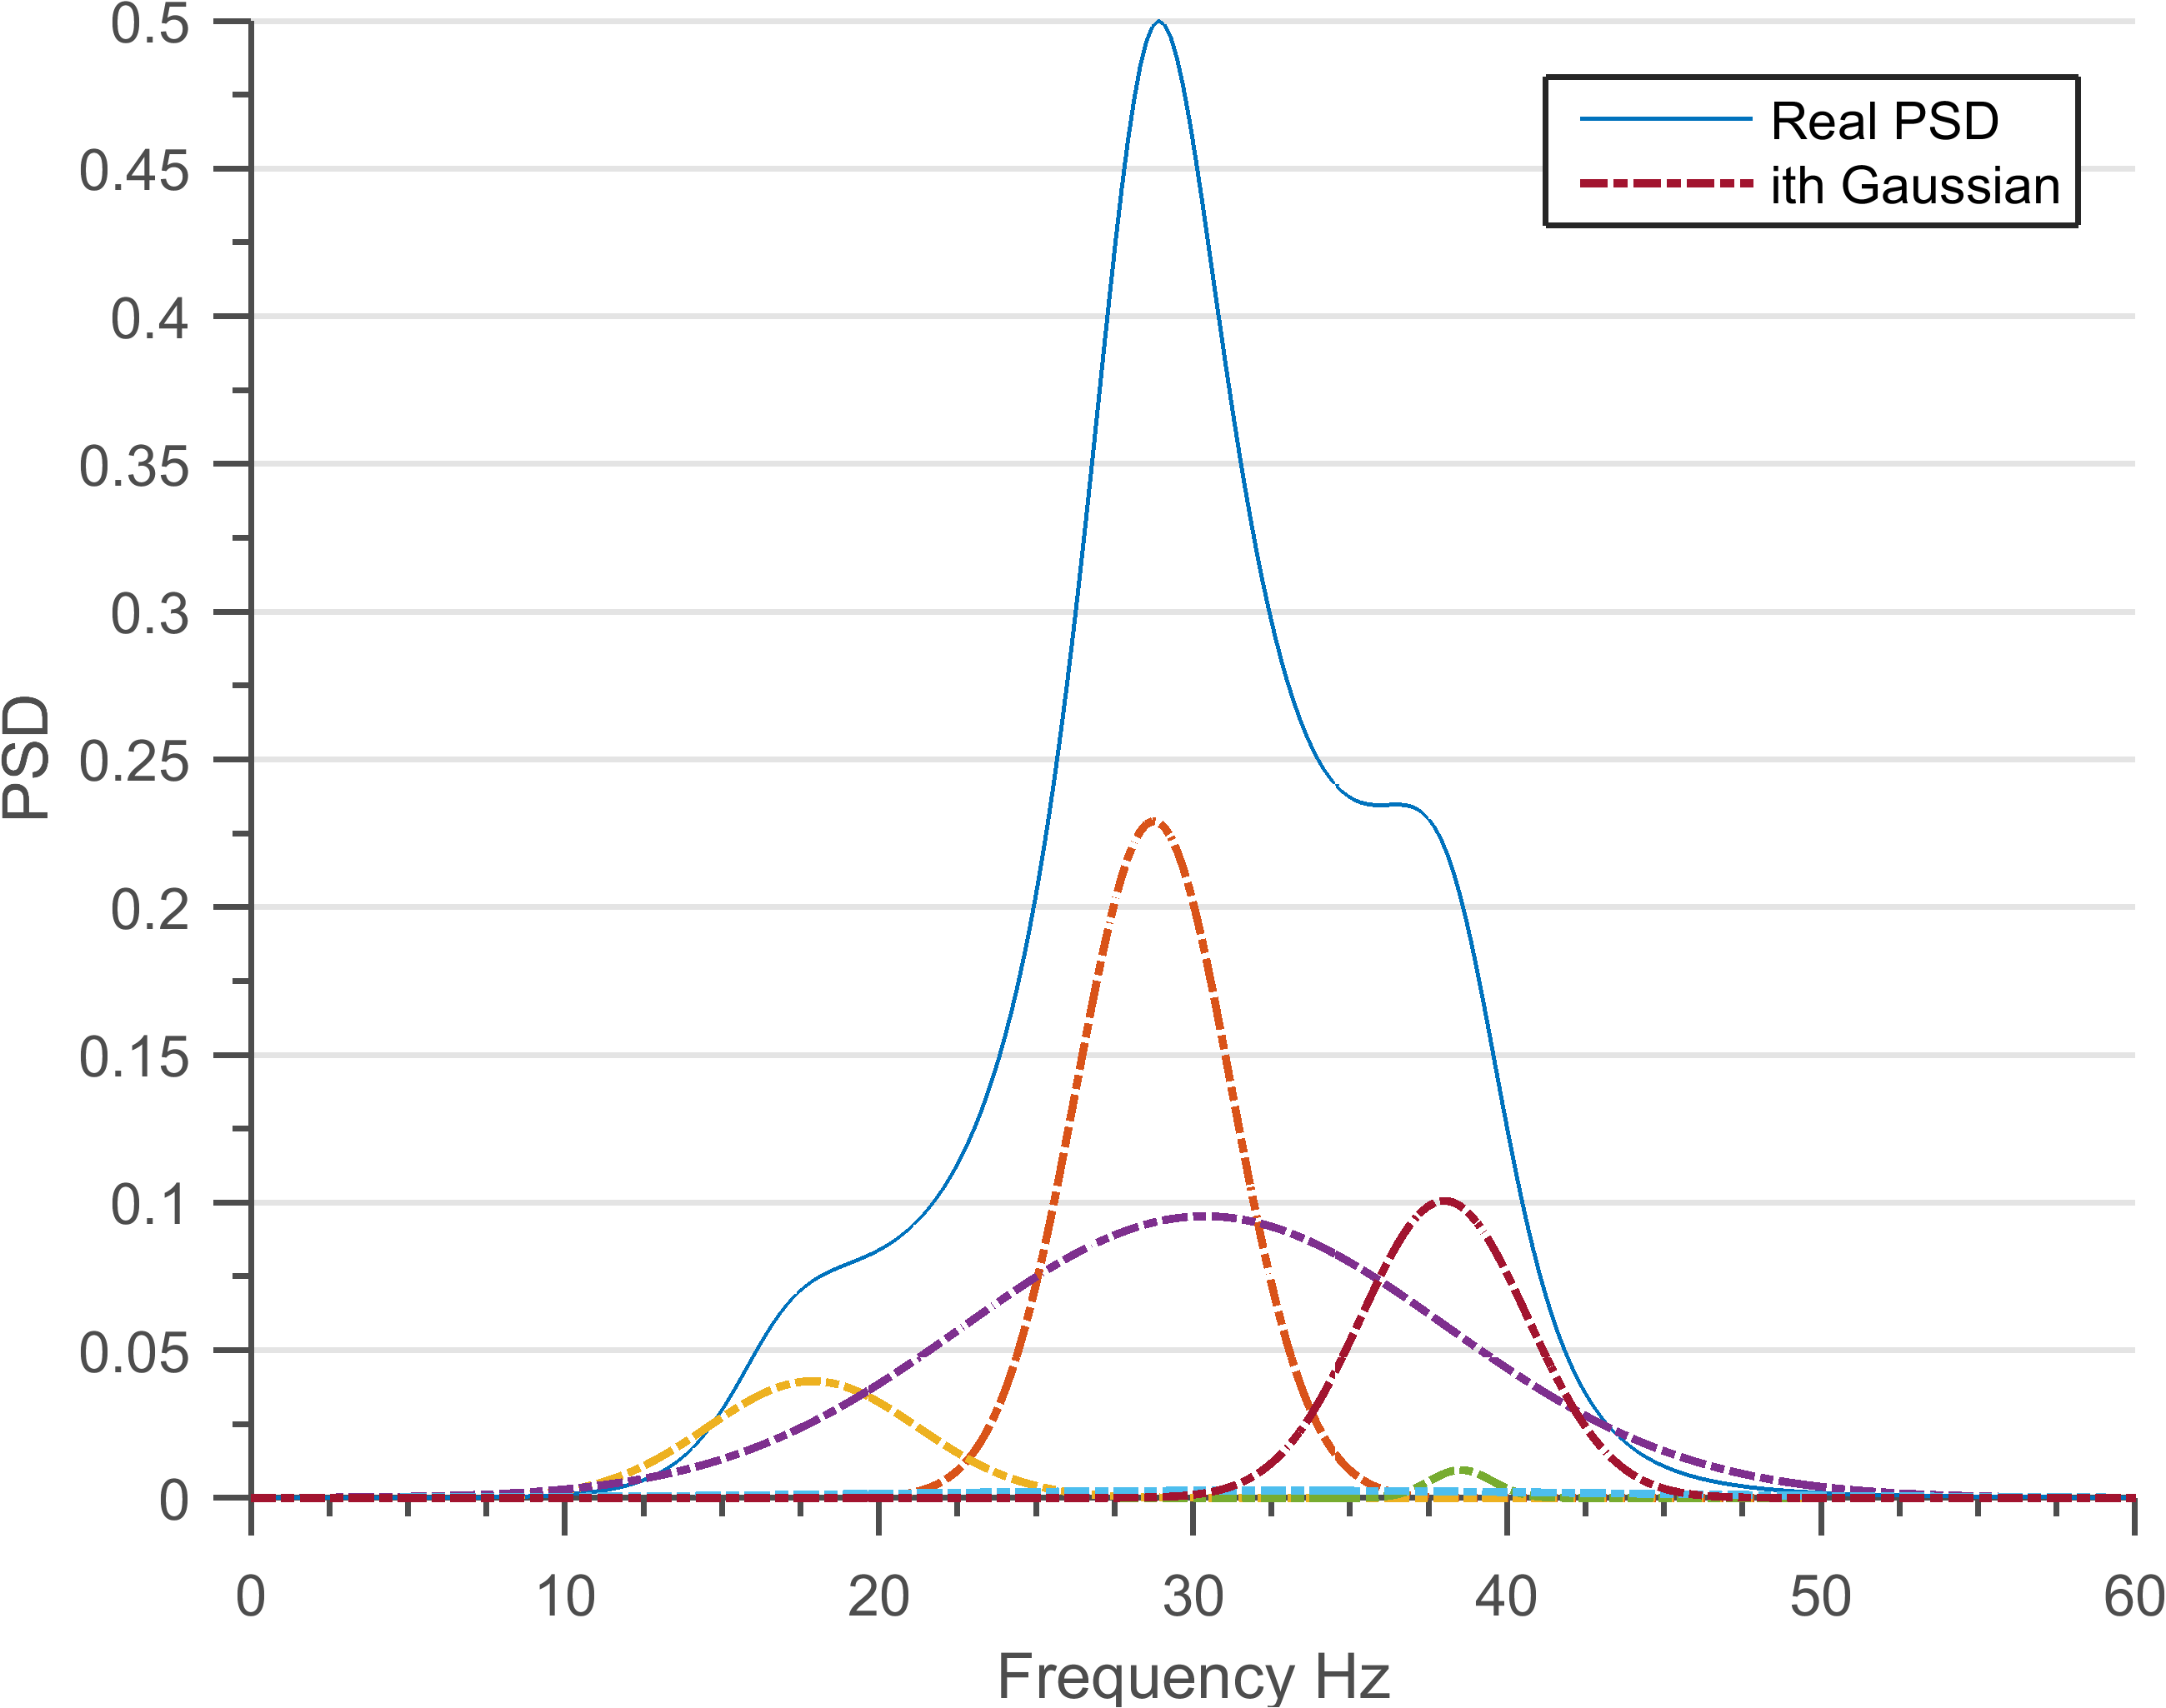
\includegraphics[width=0.3\textwidth]{images/distriButionOfGaussians}\label{subfig:distriButionOfGaussians}}

Figure \ref{subfig:stabilizationDiagram} shows the stabilization diagram with increasing number of gaussians $Q$. We can observe that as the number of $Q$ increases the algorithm starts finding better and better modes. We can also observe that there are three modes which start stabilizing from $Q=5$. The, figure \ref{subfig:bicVsQ} shows the BIC criterion with increasing number of gaussian's $Q$. We can see that that the BIC is minimum for $Q=6$ and hence if we add anymore gaussian's for our dataset we will be performing over-fitting.

Figure \ref{subfig:distriButionOfGaussians} shows the $6$ constituent gaussians which represent the $Q=6$ case. The three principal peaks represent the modal frequencies of the system, these correspond to the stabilized frequencies from figure \ref{subfig:stabilizationDiagram}. The remaining three peaks are there to compensate for the spectral density not explained by the three principal peaks. 

In the current setting of the GMM model we only propose a quick and easy way to identify the most important frequencies of a structural system. Neither the mode shapes nor the damping ratios are estimated in the current format. As can be observed from figure \ref{subfig:distriButionOfGaussians} the mode shapes are not only dependent on the principal gaussian's but also on the neighbouring gaussian's. Since some part of the spectral density is defined by non-stabilized gaussian's, in future we would like to derive a method to estimate mode-shape and damping ratio such that the contributions of neighbouring gaussian's are also taken into account.
  
  \caption{Results of applying GMM on a Spectral density}
\end{figure*}

In this paper we have proposed to identify model frequencies of a system by curve-fitting a mixture of gaussians in the frequency domain. While the common assumption that the structure can be modelled as a MDOF second order differential system causes stability issues in presence of non-linear systems. The GMM model is mathematically stable, gives results in seconds and can fit a function upto arbitrary accuracy. Moreover we introduce the BIC to identify the optimum number of gaussians and perform a trade-off between accuracy of fit and over-fitting. 

Without doubt this is very nascent stage of application of GMM for system identification and there remains problems such as identification of mode-shape and damping ratio in this algorithm. We wish to tackle these problems in the future. We also wish to apply the algorithm on a real world dataset and compare with respect to other time domain and frequency domain techniques.


\subsection{Multiplying Kernels} \label{subsec:structureKernelsMultiplyingKernels}
Since kernels should be positive semi-definite any linear operation on a kernel still results into a valid kernel. This means that multiplying two kernels also leads into a valid kernel \cite{bishop2006pattern} \cite{mackay2003information}. Multiplying two functions acts as an AND operator, the resulting kernel has high value only if we have high value on both the kernels. Multiplying any kernel with a linear kernel will introduce locality into the function , fig: \ref{subfig:SEProd2Dimensions} is a product of a linear kernel and a SE kernel it has low values where the value of linear kernel is low.

Multiplying two kernels is not only limited to a single input dimension. One can multiply kernels across several input dimensions. The multi-dimensional Automatic Relevance Determination (ARD) kernel in equation \ref{eq:SEARD} can be looked as a multiplication of several one-dimensional kernels with different length-scales. Fig: \ref{subfig:SEProd2Dimensions} is an example of a 2D SE kernel.

\begin{equation}\label{eq:SEARD}
k_{\textrm{SE}}(x, x') = \sigma^2\prod_{i=1}^{M}\exp\left(-\frac{(x - x')^2}{2\ell_{i}^2}\right)
\end{equation}

\textbf{add figure for product of kernel draws}


\subsection{Adding Kernels} \label{subsec:structureKernelsAddingKernels}
Adding two kernels acts as an OR operator. This means that the resulting kernel will have high value if either of the two kernels have high value \cite{durrande2011additive}. This property is significantly useful in extrapolation. As shown earlier one can also add kernels across dimensions, this operation encodes the information that added dimensions are independent of each other. Duvenaud \cite{duvenaud2011additive} defines a class of additive kernels which are formed upon adding several low-dimensional functions. Fig: \ref{subfig:SEAdd2Dimensions} shows addition of 2 SE kernels across dimensions, due to the OR nature extrapolation becomes easy when kernels are added.

An interesting consequence of adding kernels is that, now one can decompose the result into additive parts. This comes very handy while discovering structure in the data. Often statisticians  looks at the posterior error variance and try to add new kernels until the point such that posterior error variance represents a white noise \cite{duvenaud2013structure}, \cite{lloyd2014automatic}. 

\textbf{add figure for addition of kernel draws}

%\begin{figure}[!ht]
%  \centering
%    \subfloat[Adding SE kernels on a 2-dimensional space \label{subfig:SEAdd2Dimensions}]
%	    {\includegraphics[width=0.45\textwidth]{images/SEAdd2Dimensions}
%	   }
%	    \quad
%    \subfloat[Draws from an addition of Periodic and Linear Kernel \label{subfig:periodicPlusSEDraws}]
%	    {\includegraphics[width=0.45\textwidth]{images/periodicPlusSEDraws}
%	    }
%	    \caption{Addition of kernels}
%\end{figure}



\subsubsection{Neural Network Kernel}\label{subsubsec:nnkernel}
Neural networks have become very popular in the recent times, in the context of Gaussian Process it can be shown that a neural network with infinitely many hidden units tends to a Gaussian Process with a Neural network kernel \cite{neal2012bayesian} \cite{wilson2014covariance} equation \ref{eqnNNKernel}.

\begin{equation}\label{eqnNNKernel}
K_{NN}(x, x', \theta) = \theta_{1}^{2}\frac{2}{\pi} sin^{-1}\left ( \frac{2x\theta_{2}x'}{\sqrt{(1+2x^{T}\theta_{2}x)(1+2x'^{T}\theta_{2}x')}} \right )
\end{equation}

The hyperparameters \((\theta = [\theta_{1}, \theta_{2}])\) are; amplitude \(\theta_{1}\) which defines average distance from mean and the length scale \(\theta_{2}\) which defines the wiggliness of functions. The Neural network kernel in equation \ref{eqnNNKernel} defines a family of functions superimposed sigmoidal functions. We can use this kernel to embed the information of discontinuity in our family of functions figure \ref{subFigNNPrior}. 

\subsubsection{Application: using neural network kernel to interpolate pressures in transonic regime}
A common method of interpolating in the aerospace industry is through the use of look-up tables \cite{ghoreyshi2009accelerating}. Look-up tables encode the assumption of linearity between two data-points, thereby requiring many simulations to interpolate properly. The linearity assumption also leads to differentiability issues in higher dimensions \cite{campbell2003history}. Another popular method of surrogate modelling is by interpolating Reduced Order Models (ROM). A set of aerodynamic pressure snapshots is generated by a varying parameters, then an orthogonal linear subspace is found for these set of pressures snapshots. Generally, Proper Orthogonal Decomposition (POD) \cite{tan2003proper}, Principal Component Analysis (PCA) \cite{rosenbaum2013efficient} or Singular Value Decomposition (SVD) \cite{braconnier2011towards} are used to find the linear subspace. Finally, the reduced models are interpolated at the desired point in the parameter-space \cite{beckert2001multivariate}, \cite{barrault2004empirical}. 

Due to the assumption of linear subspace, interpolation through ROM is highly efficient both in terms of cost and performance in the subsonic regime \cite{verveld2016reduced}. Unfortunately in the transonic regime, the shock creates a highly non-linear, almost discontinuous pressure distribution and the assumption of linear subspace does not hold \cite{li2016performance}. Although performance of ROM interpolators can be improved with larger number of samples \cite{franz2014interpolation}, \cite{forrester2008engineering}, we propose to use Gaussian Process Regression \cite{rasmussen2006gaussian} keeping the same number of samples. A Gaussian Process (GP) is a distribution over functions, providing a probabilistic framework to define a family of functions. Low-level assumptions such as differentiability or smoothness can be easily encoded in GP, this enables to learn highly non-linear functions from lesser data. Moreover, using a neural network kernel \cite{neal2012bayesian} prior information of discontinuity can be embedded in GP's section \ref{subsubsec:nnkernel}. We propose to use the neural network kernel in the transonic regime to accurately predict the position and intensity of shock. 

Let us start by defining a \(3\) dimensional spatial vector \(\omega_{i} \in  \mathbb{R}^{3}\) and a \(D\) dimensional parameter space vector \(d_{j} \in  \mathbb{R}^{D}\). Such that \(\omega_{i} = \{(\omega_{i}^{1}, \omega_{i}^{2}, \omega_{i}^{3})\}\) for \(i \in [1,N_{nodes}] \) are the spatial coordinates of the \(i^{th}\) pressure node in a CFD mesh containing \(N_{nodes}\) number of pressure nodes. Whereas, \(d_{j} = \{(d_{j}^{1}, d_{j}^{2}, \ldots ,d_{j}^{D})\}\) for  \(j \in [1,N_{parameter}] \) correspond to the \(j^{th}\) parameter set. Here the parameters can be any non-spatial parameter which is desired to be interpolated upon, some common examples include Mach, Angle of Attack for steady aerodynamics and time or frequency for unsteady aerodynamics. Since, this paper relates to interpolating steady aerodynamics \(d_{j}\) will correspond to the \(j^{th}\) CFD run in a total of \(N_{parameter}\) CFD simulations.

We now proceed to compare the accuracy of two methods in transonic regime on Common Research Model (CRM)  proposed by NASA. Since the introduction of the model for the 4th Drag Prediction Workshop, the CRM has been become a very widely used test case for applied computational aerodynamics. Due to the widespread experience and availability of wind-tunnel test results for the configuration this is a natural case to benchmark interpolations. We compare the accuracy on CRM wing in the transonic regime using elsA solver and kOmega-SST turbulence model as prescribed by airbus during the fourth drag prediction workshop \cite{vassberg2014summary}. 

\begin{figure*}[!ht]
  \centering
  \subfigure[{Common research model. The four red lines are the four cuts at \(y/b = [0.105, 0.37, 0.5, 0.84]\)}.]
  {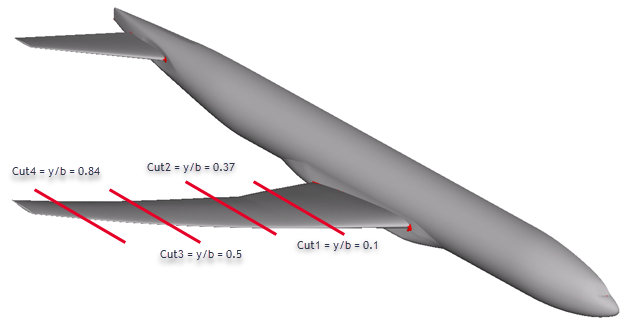
\includegraphics[width=0.45\textwidth]{images/crm_Wing_design}\label{subfig:crmWing}}\quad
    \subfigure[{Pressure snapshot on the Common Research model for \(\alpha = 2\) and \(Mach = 0.85\)}]
    {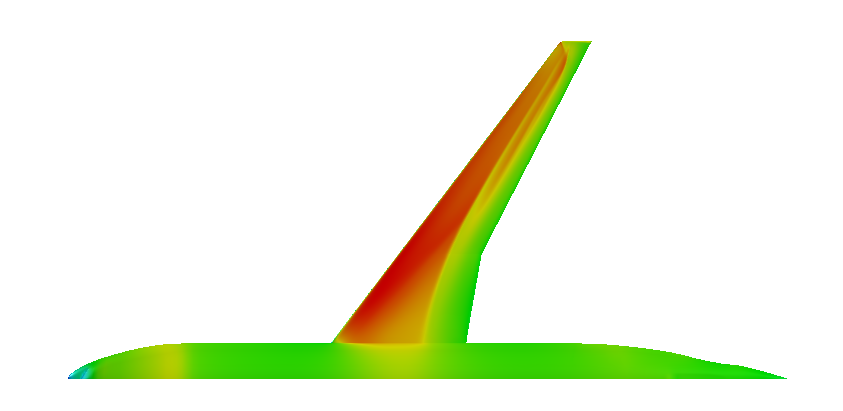
\includegraphics[width=0.45\textwidth]{images/surfM85A2}\label{subfig:crmSnapshot}}
  \caption{Common Research Model}
\end{figure*}

Again we use the elsA\textsuperscript{\textregistered} solver to perform simulations on the design. We use the \(\kappa - \omega\) SST turbulence model to perform predictions since it has good performance in the fuselage wing interaction regions \cite{menter2003ten}, \cite{vassberg2014summary}. The CFD was run for a combination of 21 values of \(\alpha \in [1: 0.1: 3]\) and 5 values of \(Mach \in [0.84: 0.005: 0.86]\), hence \(N_{parameter} = 21\times5 = 105\). Figure, \ref{subfig:crmSnapshot} shows one of the pressure snapshots for \(\alpha = 2\) and \(Mach = 0.85\). We then cut the wing at four distinct locations \(y/b = [0.105, 0.37, 0.5, 0.84]\) to clearly observe different types of airfoil behavior, figure \ref{subfig:crmWing} is the CRM location of four cuts. 

As detailed in the earlier section we again use LOO for comparing the performance of two methods. The POD+I method has been run as described in section \ref{sec:podi}. The distributed GP has been run as described in the earlier section only this time we use Neural Network kernel for the spatial dimension. The neural network kernel lets use encode information of discontinuity (as expected from shock) in our family of functions as detailed in section \ref{subsubsec:nnkernel}. 

We use Leave One Out (LOO) Cross Validation method to quantify the performance of the two methodologies. Here, $[\alpha, \theta]$ doublets are removed one by one from the database to create a new training set. The new training set is used to perform interpolation according to POD+I and distributed GP. Pressure snapshot is reconstructed for the missing $[\alpha, \theta]$ doublets by interpolation. The methods are finally compared by evaluating the Root Mean Square Error (RMSE) and time of prediction values for each doublet case. 

As described in section \ref{sec:podi} we use all the available modes for pressure snapshot reconstruction. While performing distributed GP regression, we learn a GP model between \(p_{ij}\) and input vector \(X = [\Omega, \alpha, Mach]\). 

\begin{figure*}[!ht]
  \centering
  \subfigure[{Normalized RMSE for the two different model types. The x axis denotes indices of removed doublets. POD has a RMSE of \(0.32\pm0.23\) whereas distributed GP has a RMSE of \(0.02\pm0.01\). The average distributed GP prediction is 16 times better than POD in transonic regime}]
  {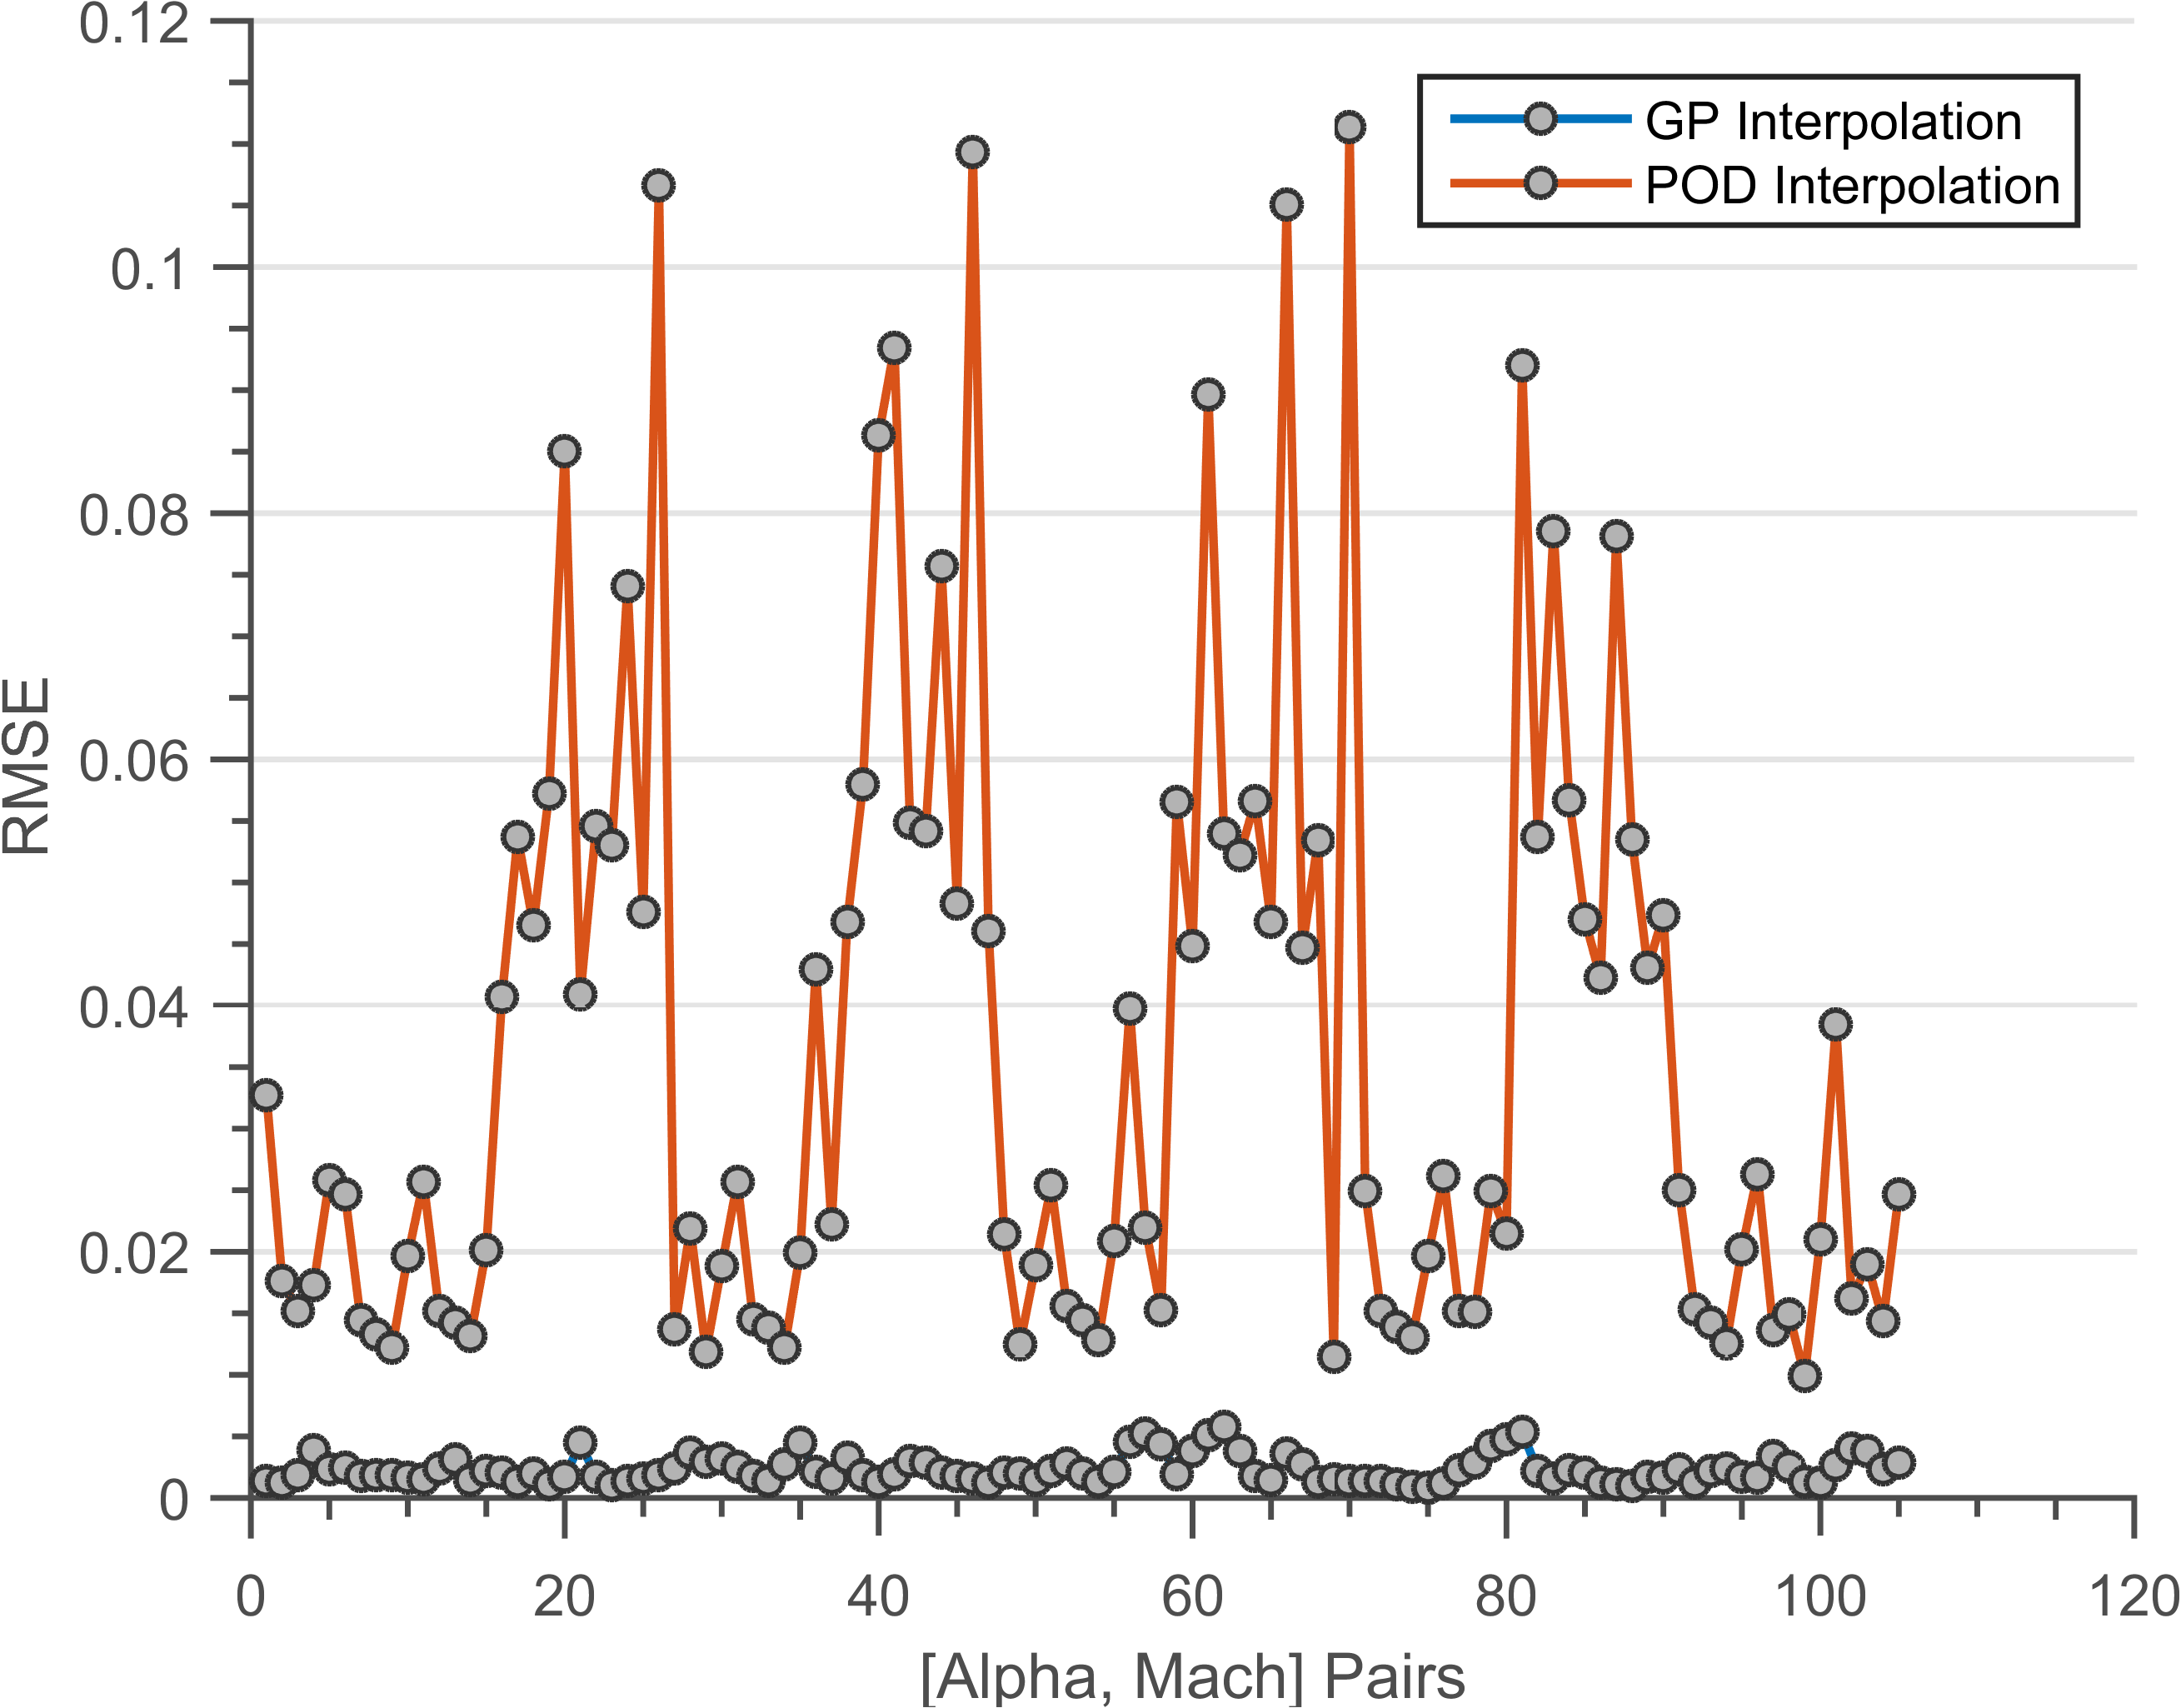
\includegraphics[width=0.45\textwidth]{images/rmseCRM}\label{subfig:RMSECRM}}\quad
    \subfigure[{Time taken to perform prediction for the two different model types. The x axis denotes indices of removed doublets. POD takes \(0.05s\pm0.003s\) whereas distributed GP takes \(4.06s\pm0.23s\) to perform the interpolation. The average POD interpolation is 80 times faster than distributed GP.}]
    {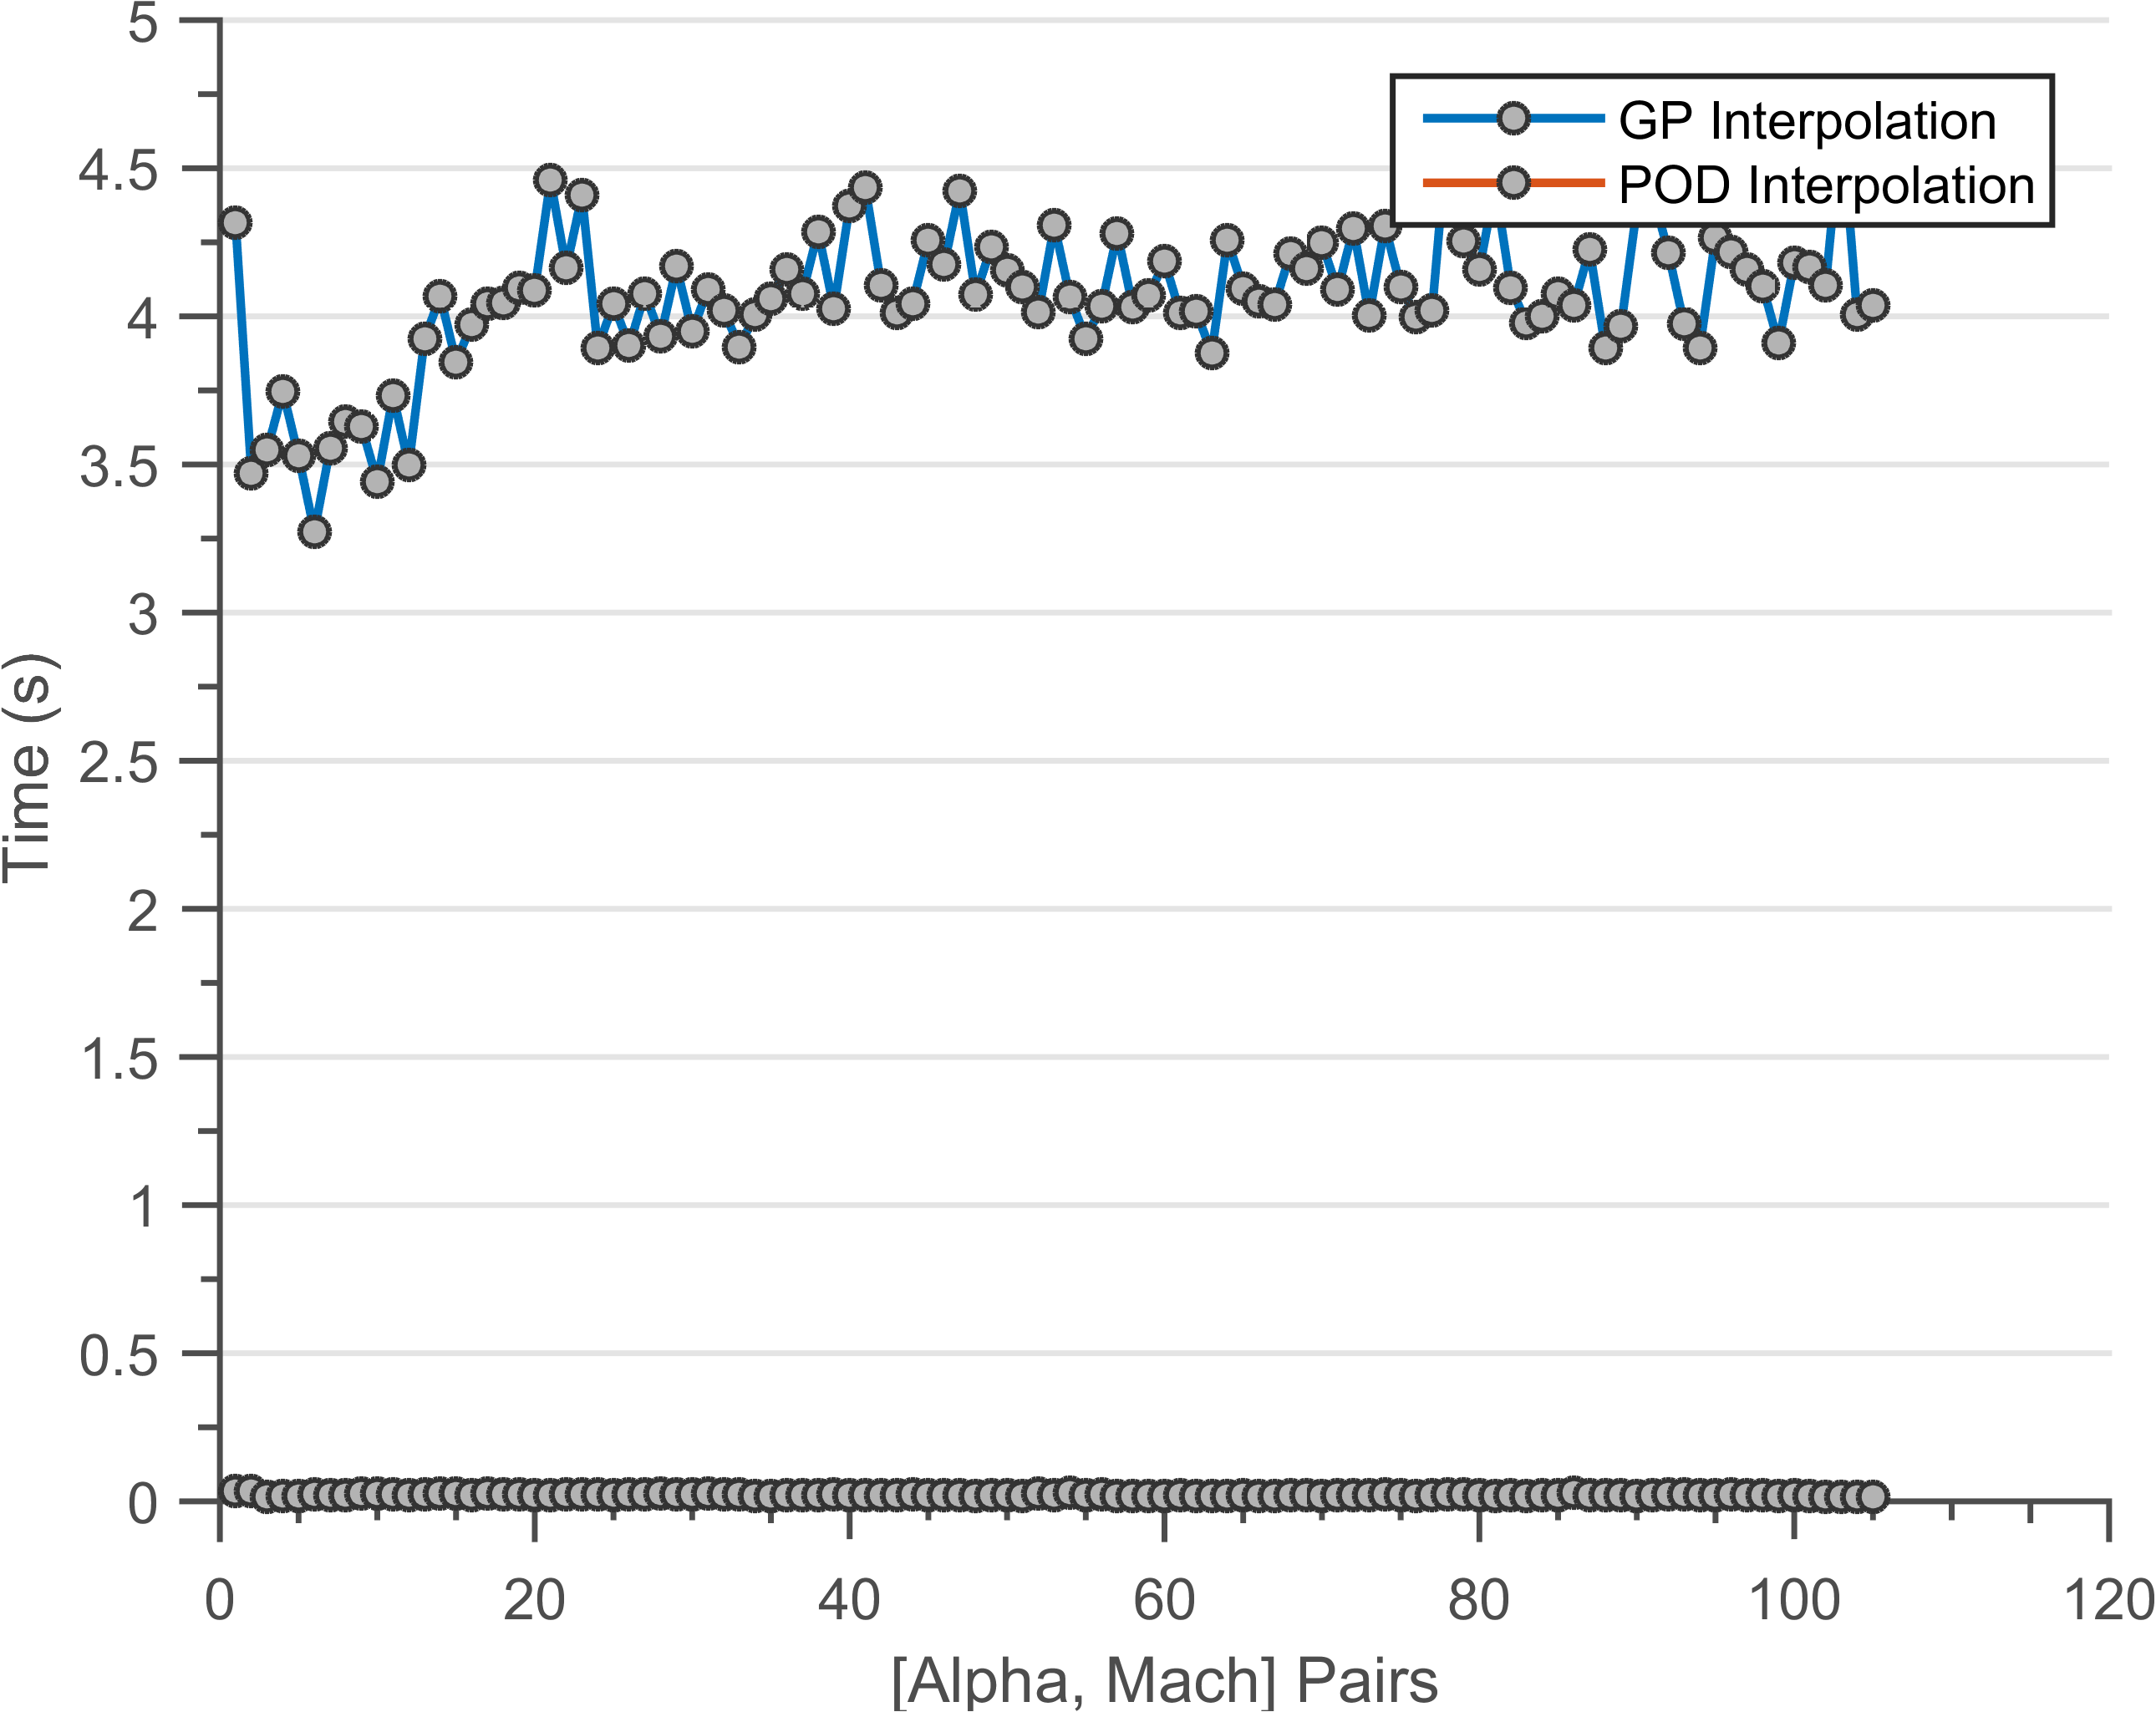
\includegraphics[width=0.45\textwidth]{images/timeCRM}\label{subfig:timeCRM}}
  \caption{Results for CRM interpolation}
\end{figure*}

The above figures \ref{subfig:RMSECRM} denote the RMSE estimates for different doublets. POD has a RMSE of \(0.32\pm0.23\) whereas distributed GP has a RMSE of \(0.02\pm0.01\). The average distributed GP prediction is 16 times better than POD in transonic regime. The peaks in the RMSE plots denote cases where the removed doublets are on the edges of database. Hence extrapolation is performed during these experiments. Figure \ref{subfig:timeCRM} shows the time taken to perform prediction for the three different model types. The x axis denotes indices of removed doublets. POD takes \(0.05s\pm0.003s\) whereas distributed GP takes \(4.06s\pm0.23s\) to perform the interpolation. In transonic regime GP has a significantly better error performance and becomes the obvious choice for interpolation.

\begin{figure*}[!ht]
  \centering
  \subfigure[{Comparison between POD interpolation and distributed GP for interpolation. Reconstruction is performed on the pressure snapshot at \(\alpha = 2\) and \(Mach = 0.85\) for the \(y/b = 0.105\)}. We can observe that the intensity of shock has been smoothed out by POD interpolation]
  {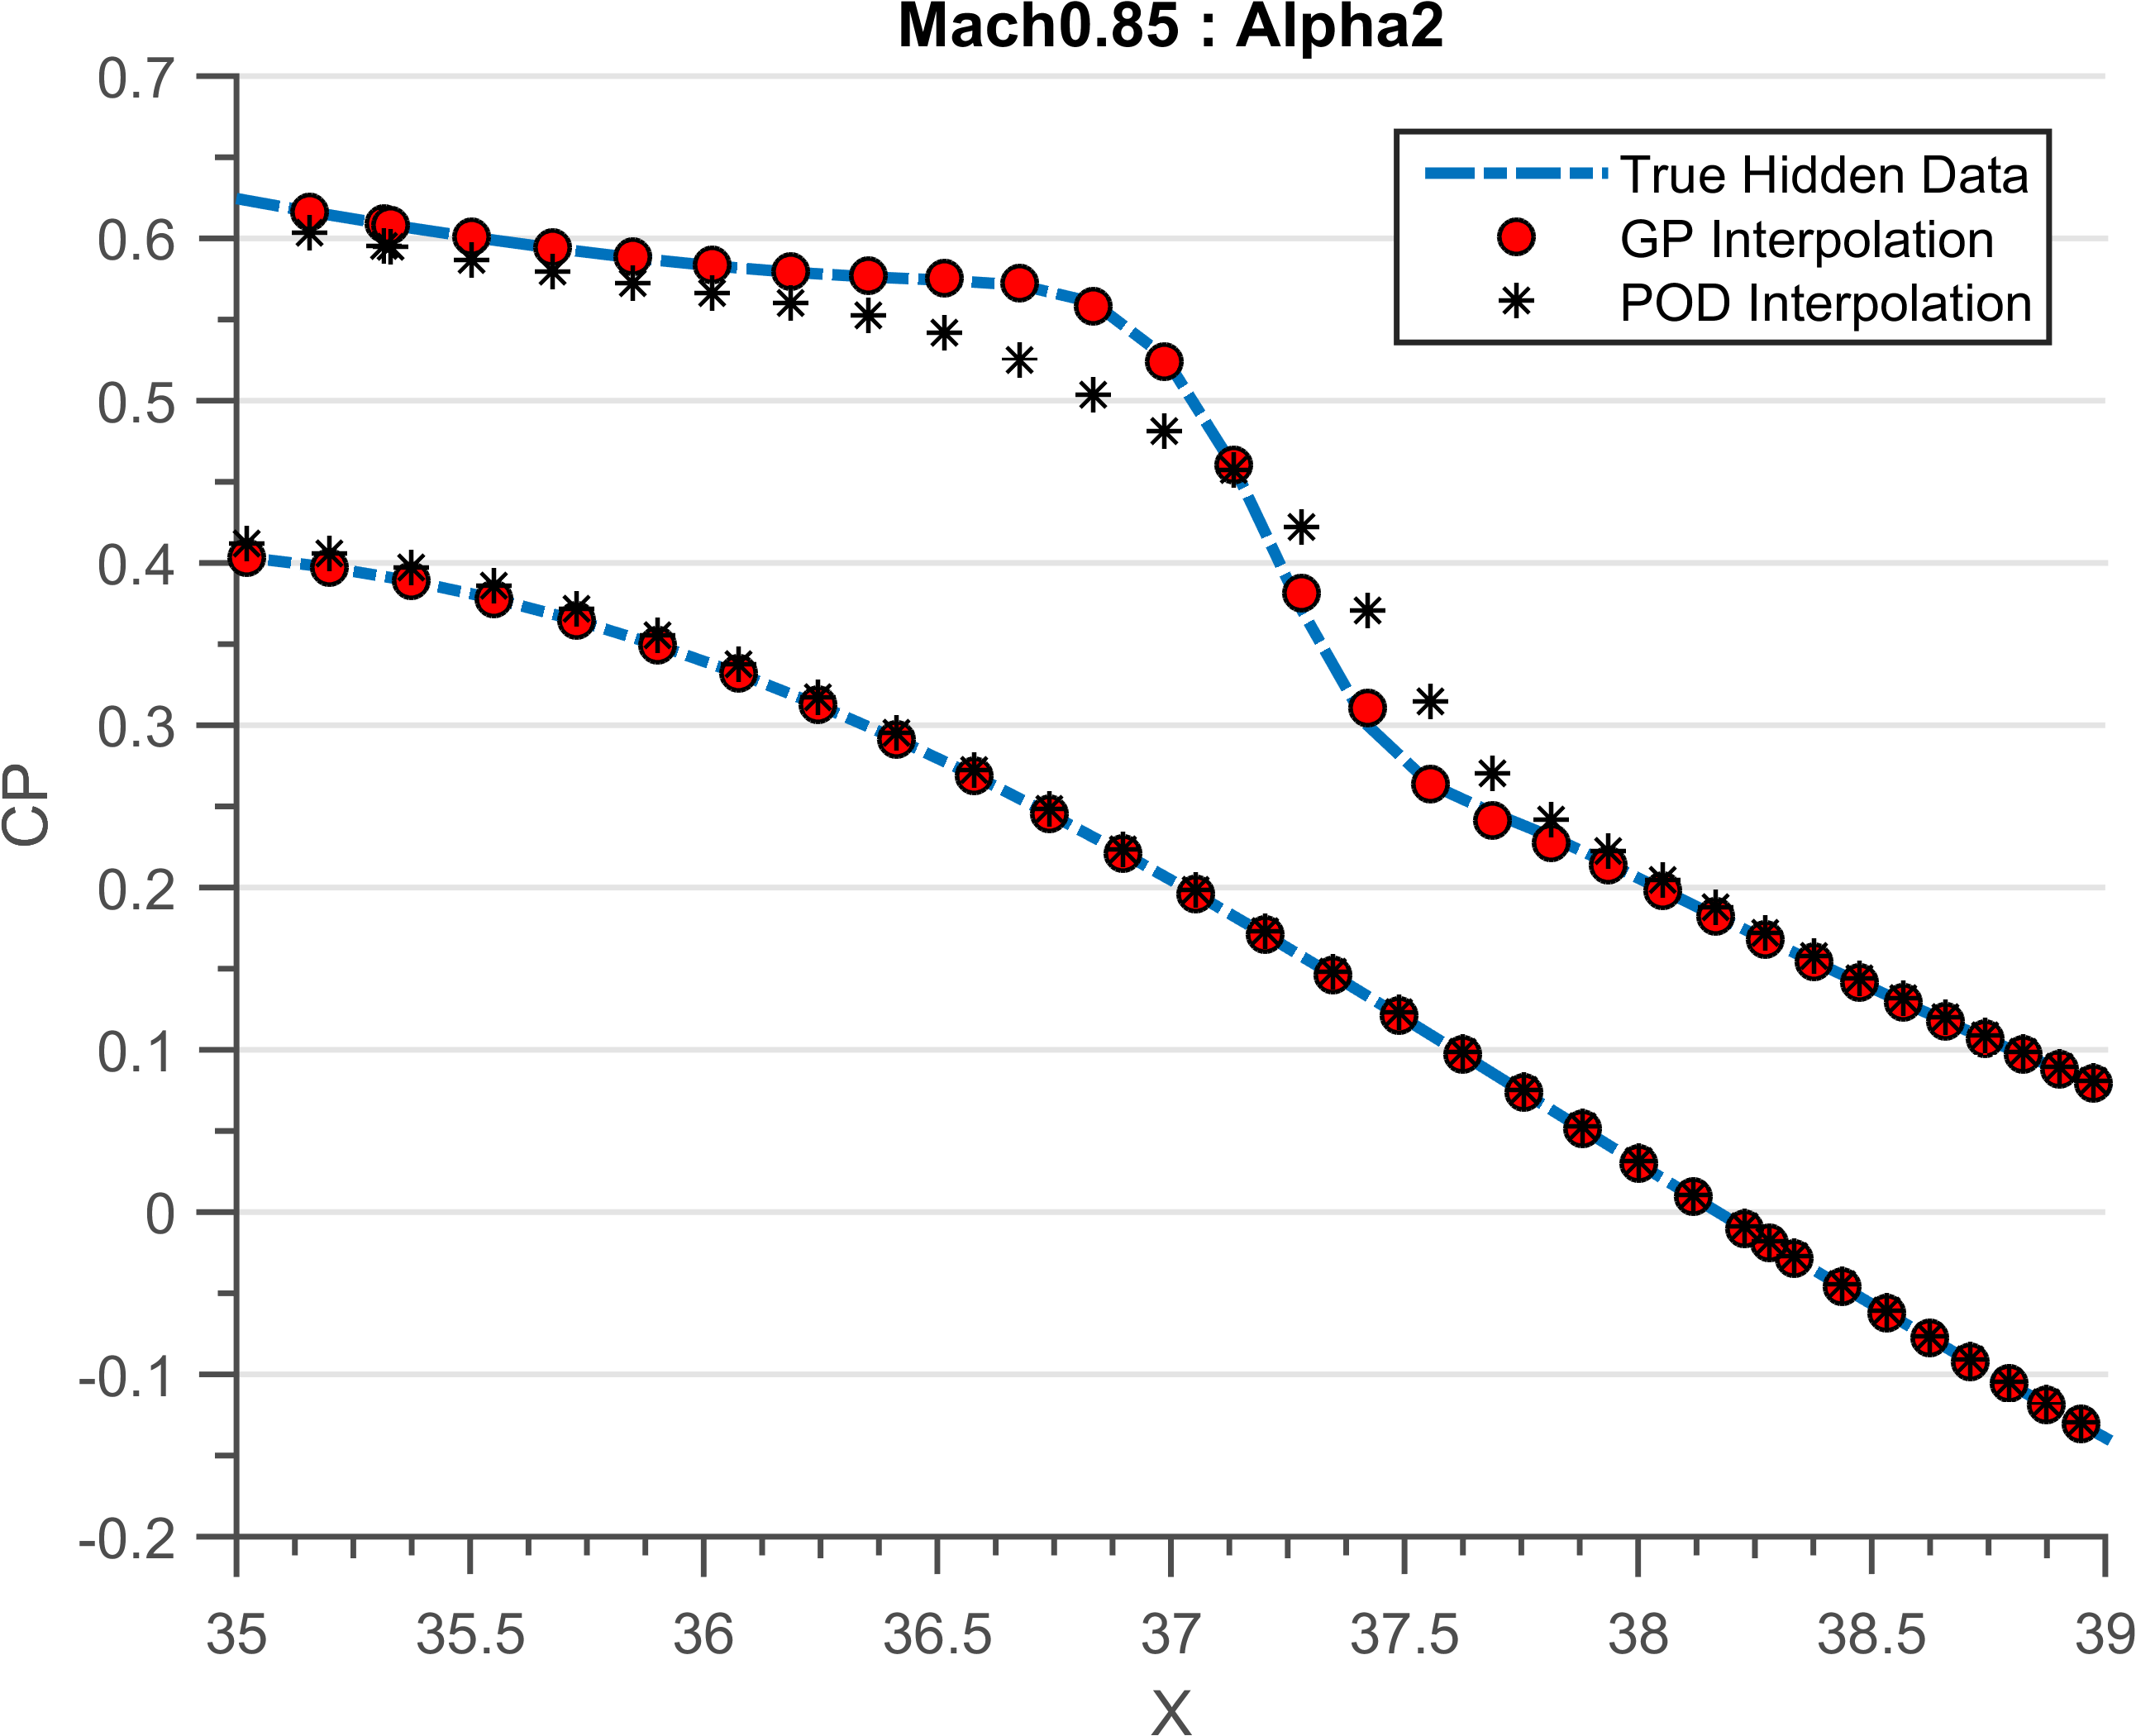
\includegraphics[width=0.45\textwidth]{images/CRM-clean-testSnapshots_M850A20}\label{subfig:interpComparisonCRM}}\quad
    \subfigure[{Comparison between POD interpolation and distributed GP for extrapolation. Reconstruction is performed on the pressure snapshot at \(\alpha = 2\) and \(Mach = 0.84\) for the \(y/b = 0.105\). We can observe that POD introduces errors both for the intensity of shock and location of shock for this case}]
    {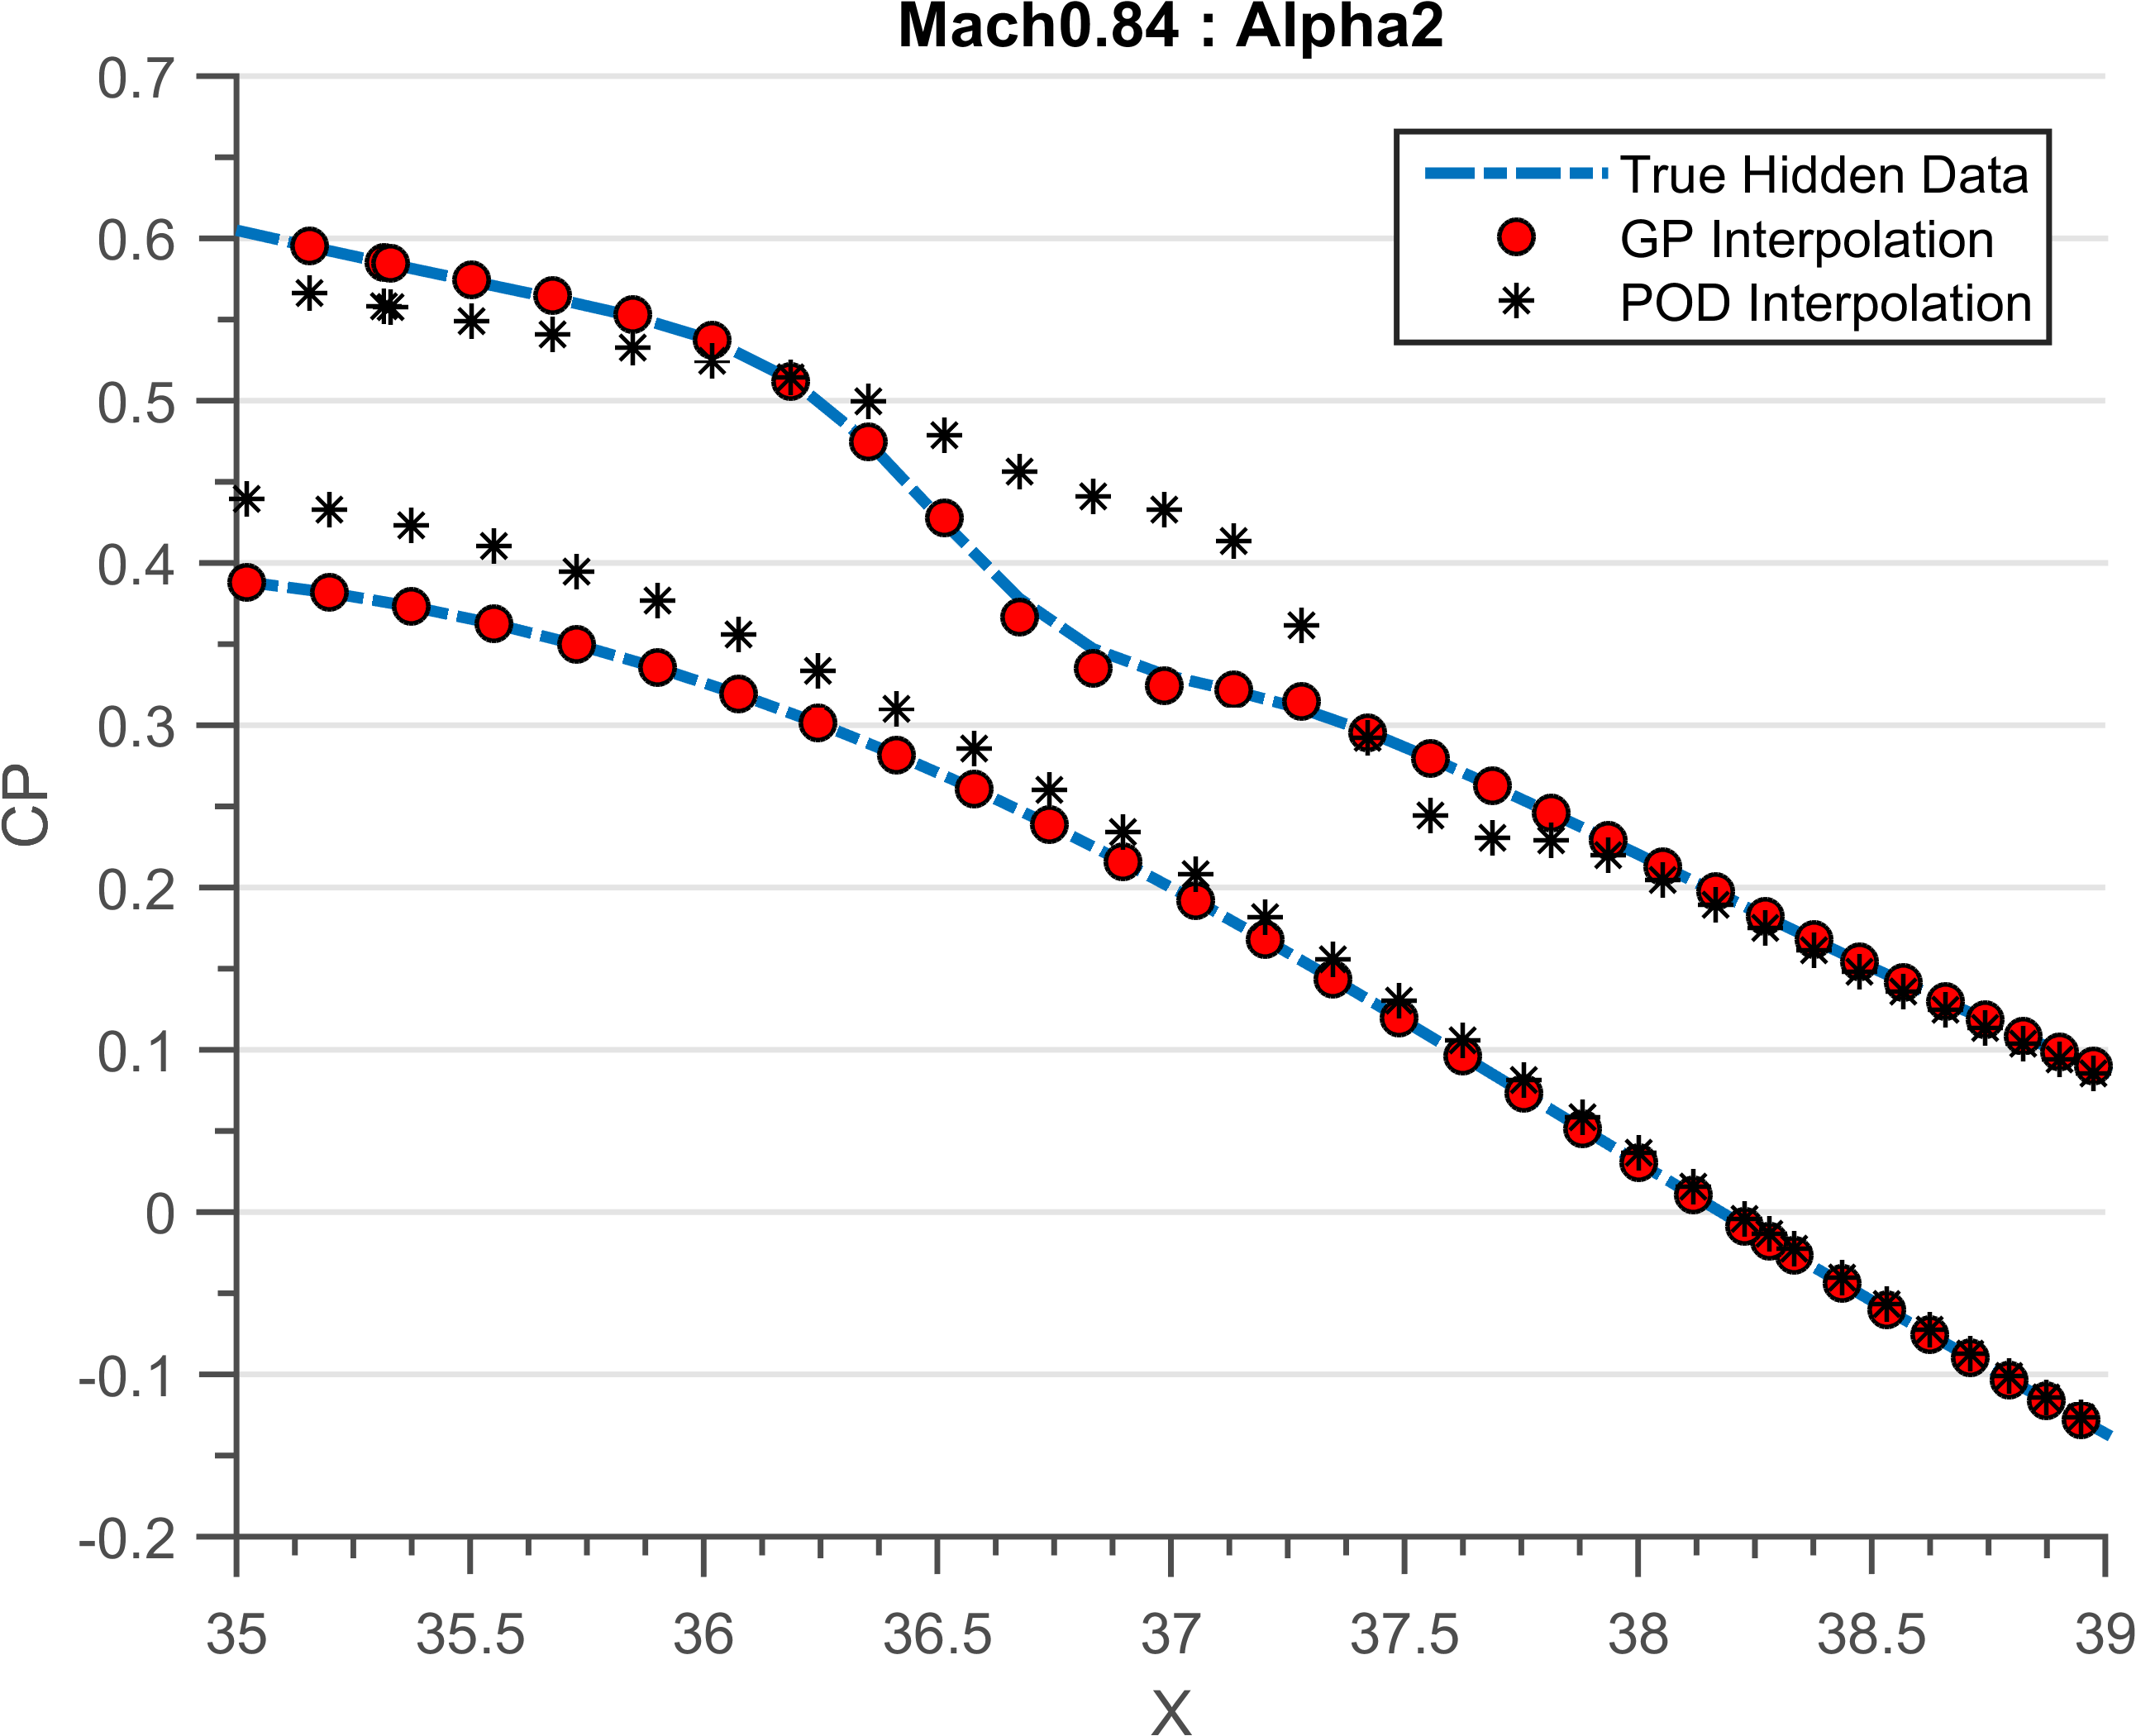
\includegraphics[width=0.45\textwidth]{images/CRM-clean-testSnapshots_M840A20}\label{subfig:exterpComparisonCRM}}
  \caption{Comparison of pressure interpolations for first cut \(y/b = 0.105\), only showing section near shock for clarity.}
\end{figure*}

Figure \ref{subfig:interpComparisonCRM} shows the comparison between POD interpolation and distributed GP for interpolation. Reconstruction is performed on the pressure snapshot at \(\alpha = 2\) and \(Mach = 0.85\) for the \(y/b = 0.105\). We can observe that the shape of shock has been smoothed out by POD interpolation. Figure \ref{subfig:exterpComparisonCRM} shows comparison between POD interpolation and distributed GP for extrapolation. Reconstruction is performed on the hidden pressure snapshot of \(\alpha = 2\) and \(Mach = 0.84\). We can observe that POD introduces errors both for the intensity of shock and location of shock for this case.  

\subsubsection{Comparison across cuts}
We next study the performance of distributed GP for different airfoils on the wing. Using the methodology described earlier we build a distributed GP model for each airfoil and measure the performance of interpolation performed for each cut using the LOO methodology. 

\begin{figure*}[!ht]
  \centering
  \subfigure[{Normalized RMSE for different airfoils based on distributed GP. The x axis denotes indices of removed doublets. The mean RMSE of different cuts from \(y/b = [0.105, 0.37, 0.5, 0.84]\) is \([0.053, 0.17, 0.31, 0.40]\) respectively. The performance of interpolation deteriorates as we go farther away from the fuselage}]
  {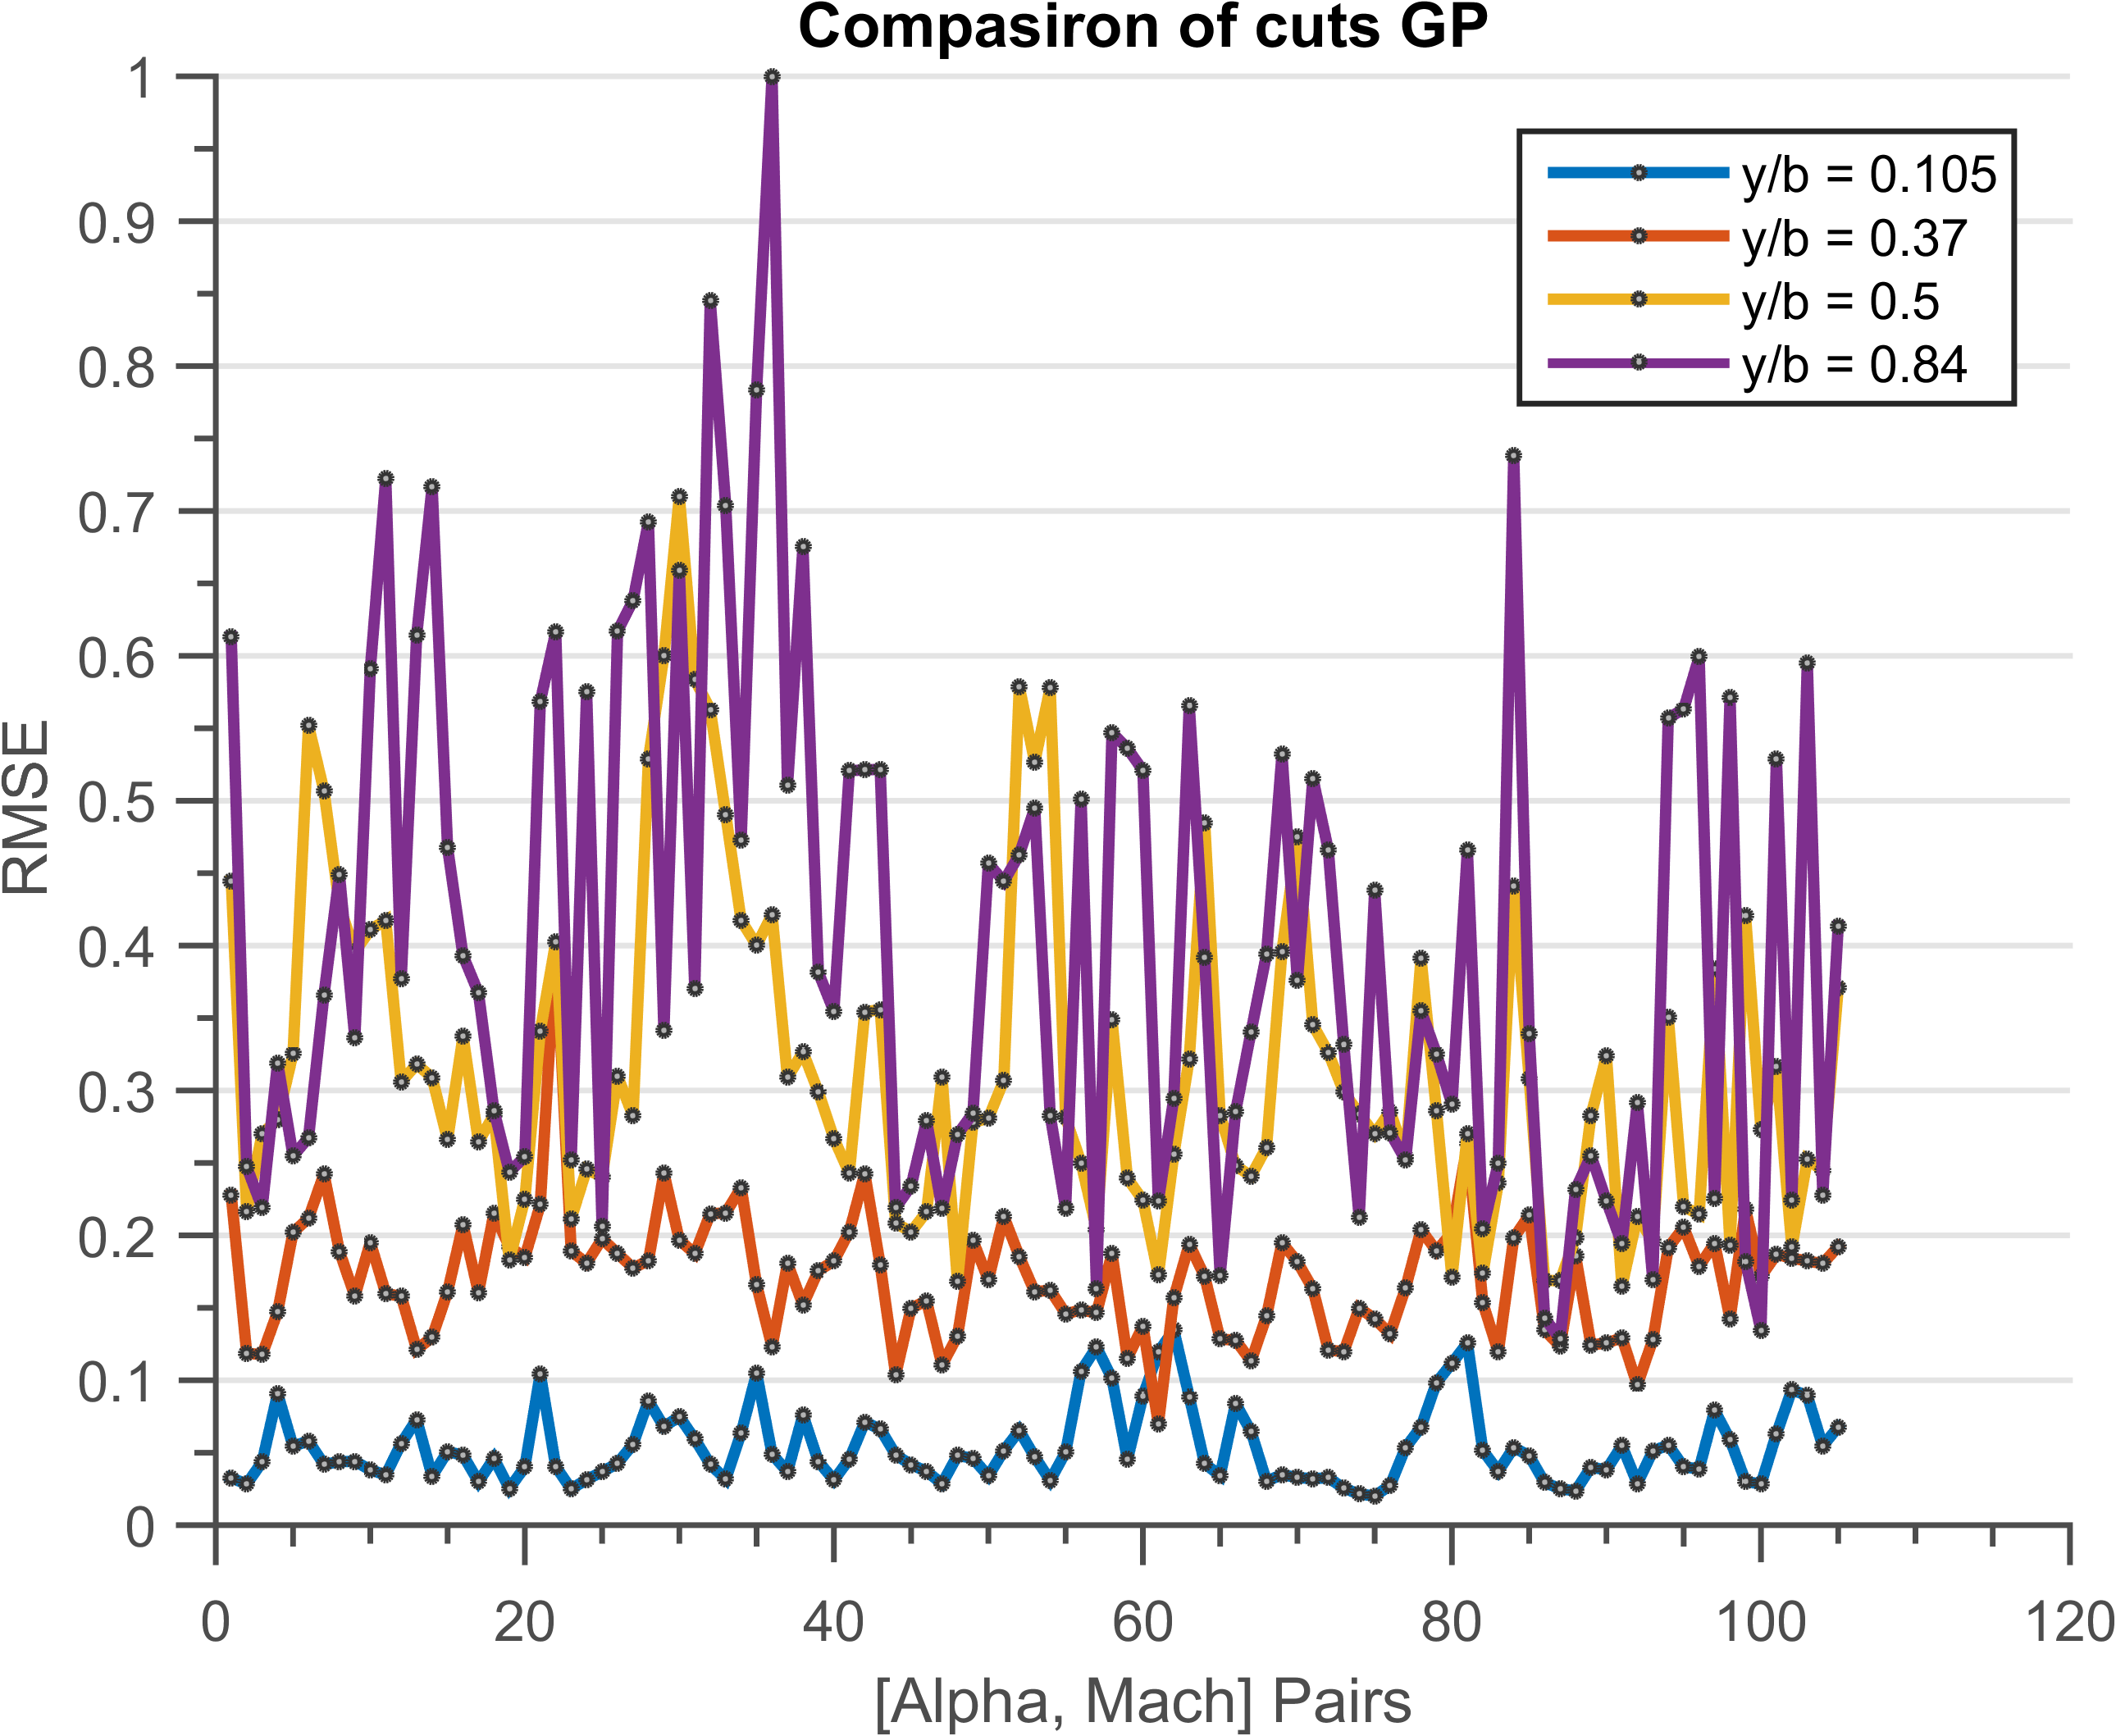
\includegraphics[width=0.45\textwidth]{images/compasironOfCutsGPCRM}\label{subfig:compasironOfCutsGPCRM}}\quad
    \subfigure[{Comparison between POD interpolation and distributed GP for interpolation. Reconstruction is performed on the pressure snapshot at \(\alpha = 2\) and \(Mach = 0.85\) for the location  \(y/b = 0.84\)}. While POD smooths out the double shock pattern distributed GP also lacks the accuracy observed in figure \ref{subfig:interpComparisonCRM}. Only showing chord location near shock for clarity.]
    {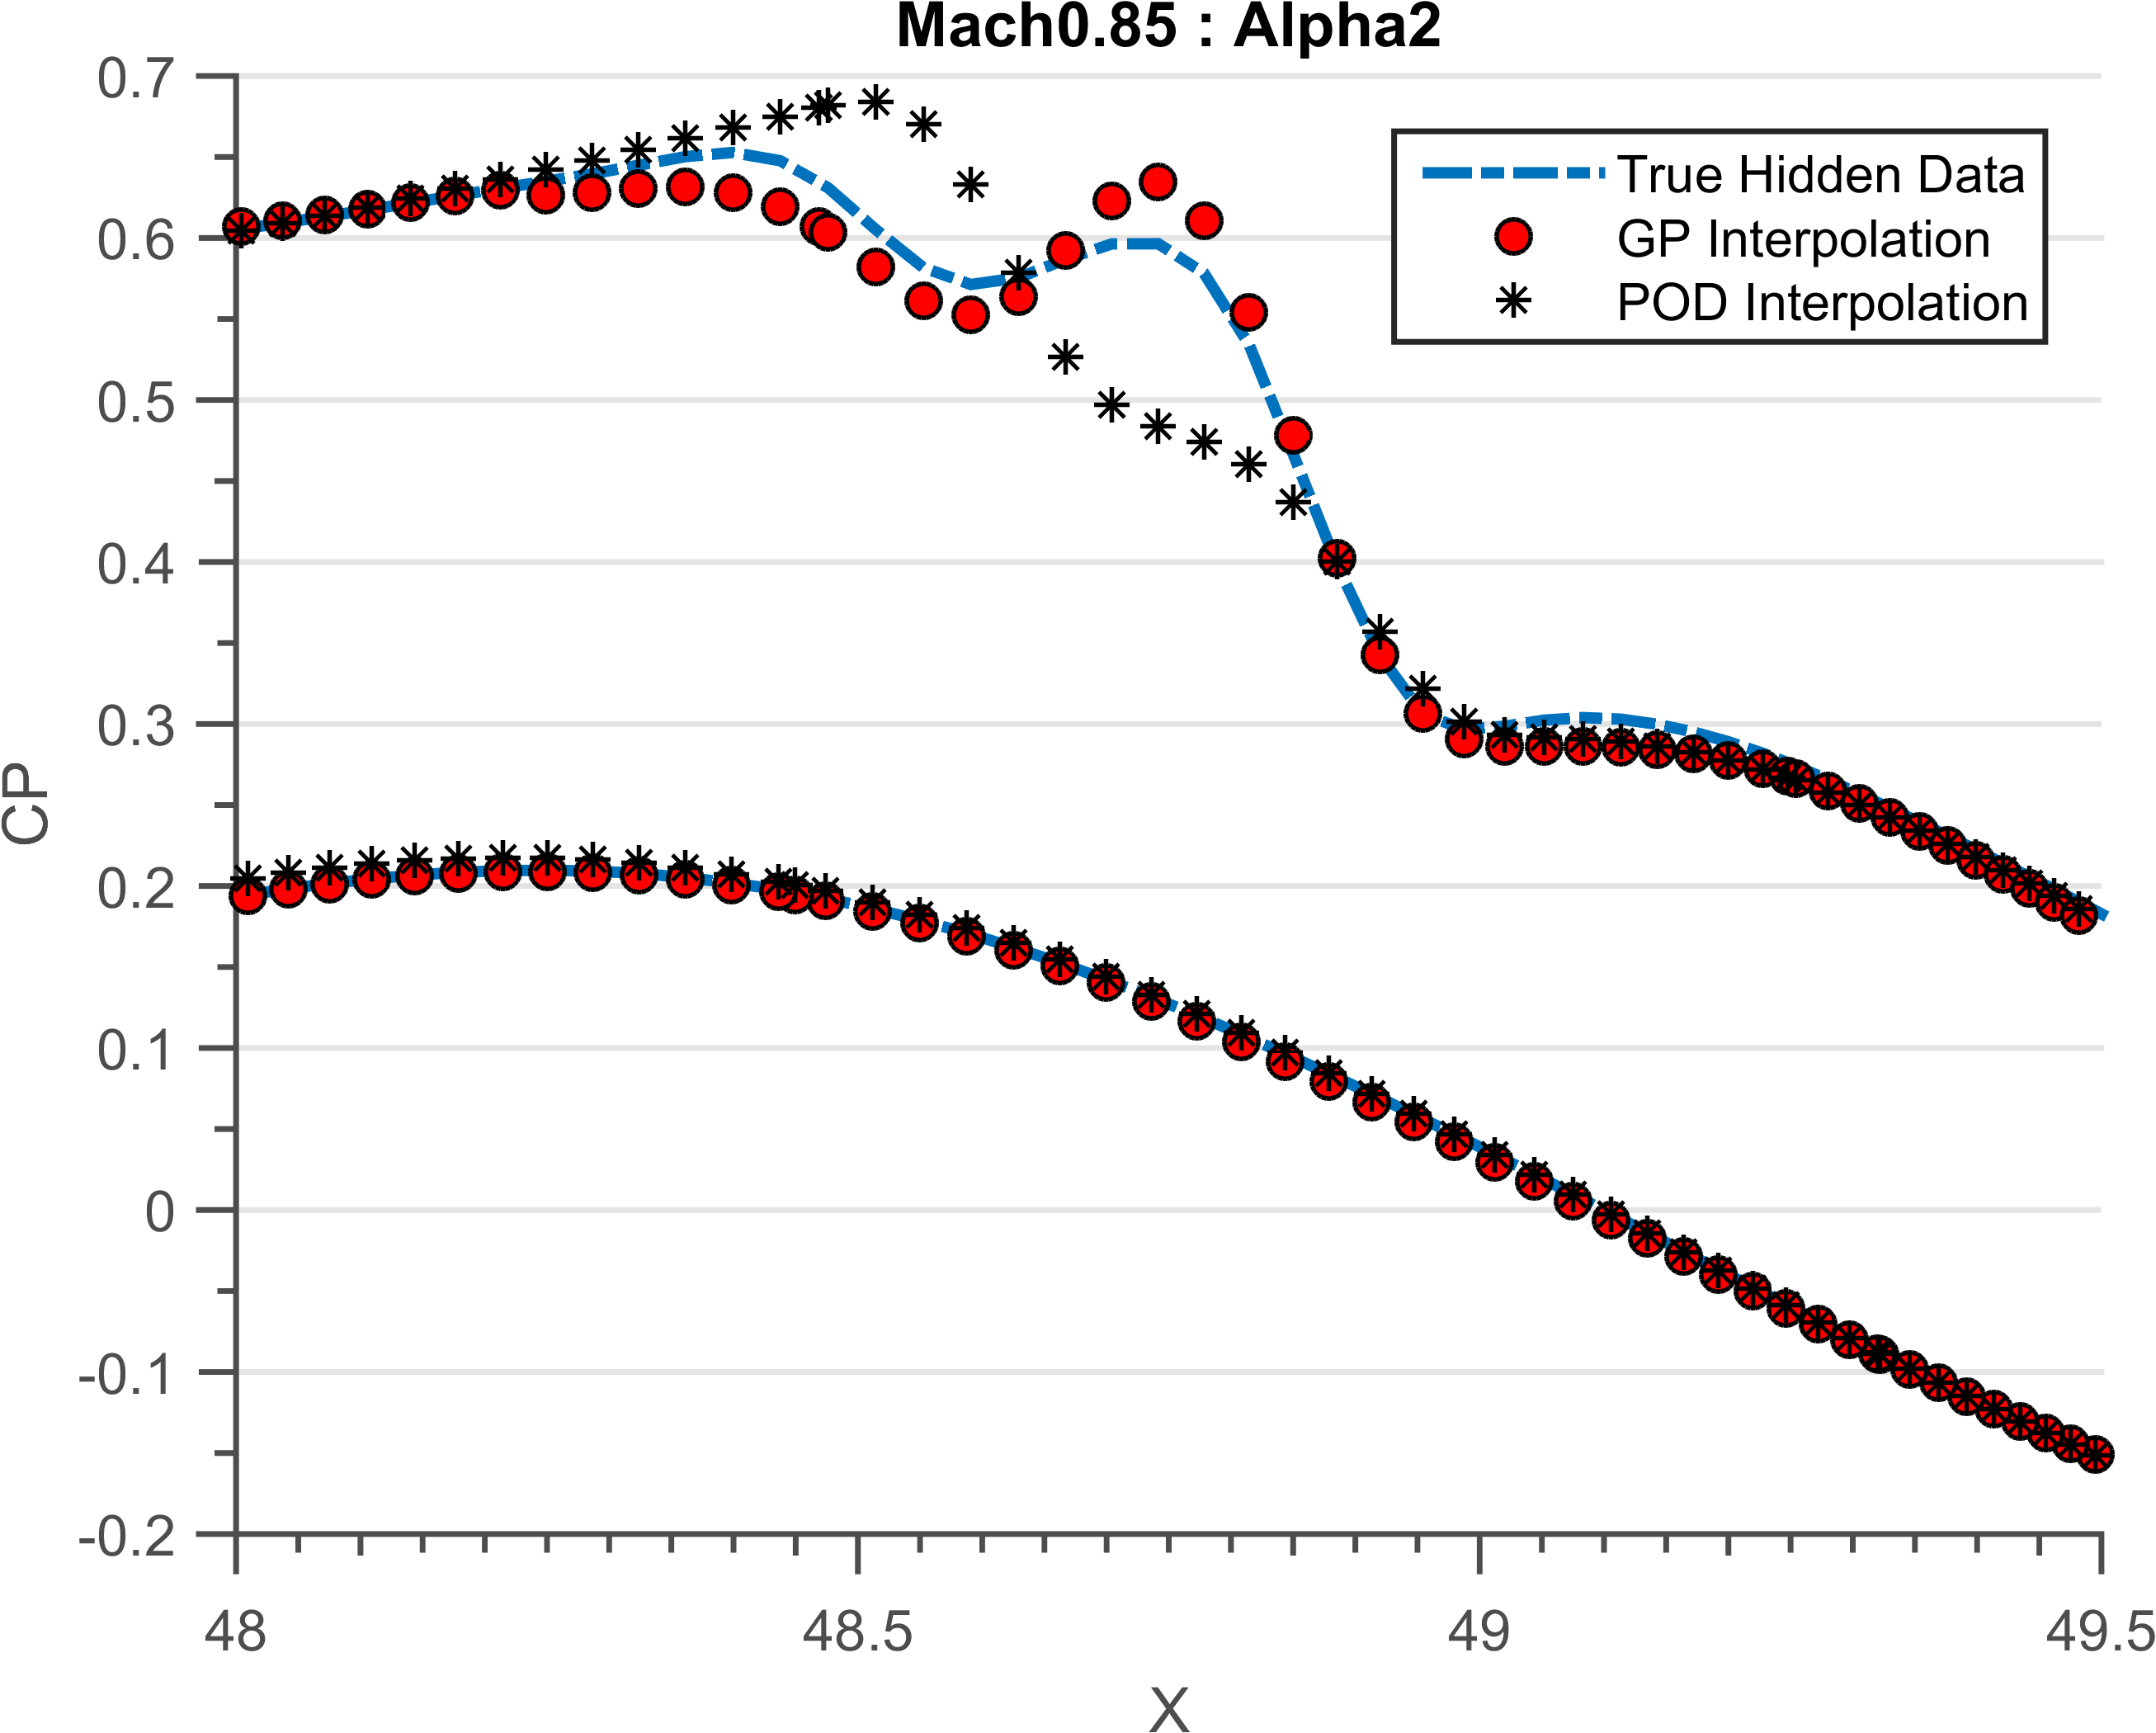
\includegraphics[width=0.45\textwidth]{images/CRM-clean-testSnapshots_M850A20_cut4}\label{subfig:interpCut4}}
  \caption{Performance of distributed GP across cuts}
\end{figure*}

Figure \ref{subfig:compasironOfCutsGPCRM} shows the RMSE performance across cuts. The x axis denotes indices of removed doublets. The RMSE of different cuts from \(y/b = [0.105, 0.37, 0.5, 0.84]\) is \([0.053\pm0.02, 0.17\pm0.04, 0.31\pm0.11, 0.40\pm0.17]\) respectively. The performance of interpolation deteriorates as we go farther away from the fuselage. This is primarily because as we go farther away from the fuselage double shocks start appearing on the airfoil figure \ref{subfig:crmSnapshot}. Figure \ref{subfig:interpCut4} shows interpolation performed by the POD interpolation and distributed GP methods at \(\alpha = 2\) and \(Mach = 0.85\). While, POD smooths out the double shock pattern distributed GP also lacks the accuracy observed in figure \ref{subfig:interpComparisonCRM}. 

\begin{figure*}[!ht]
  \centering
  \subfigure[{Interpolation performed at constant \(Mach = 0.845\) and \(\alpha = [1, 3]\) for the location \(y/b = 0.105\). The color coding denotes coefficient of pressure for upper side of airfoil, The x-axis denotes chord-wise location and y-axis denotes \(\alpha\). White lines denote presence of a pressure snapshot due to CFD run, everything in between is interpolation. Dashed black lines denote constant pressure contours color between two contours has been smoothed for clarity. We observe a strong shock near \(\alpha = 3\) which slowly gets converted to a weak shock near \(\alpha = 1\).}]
  {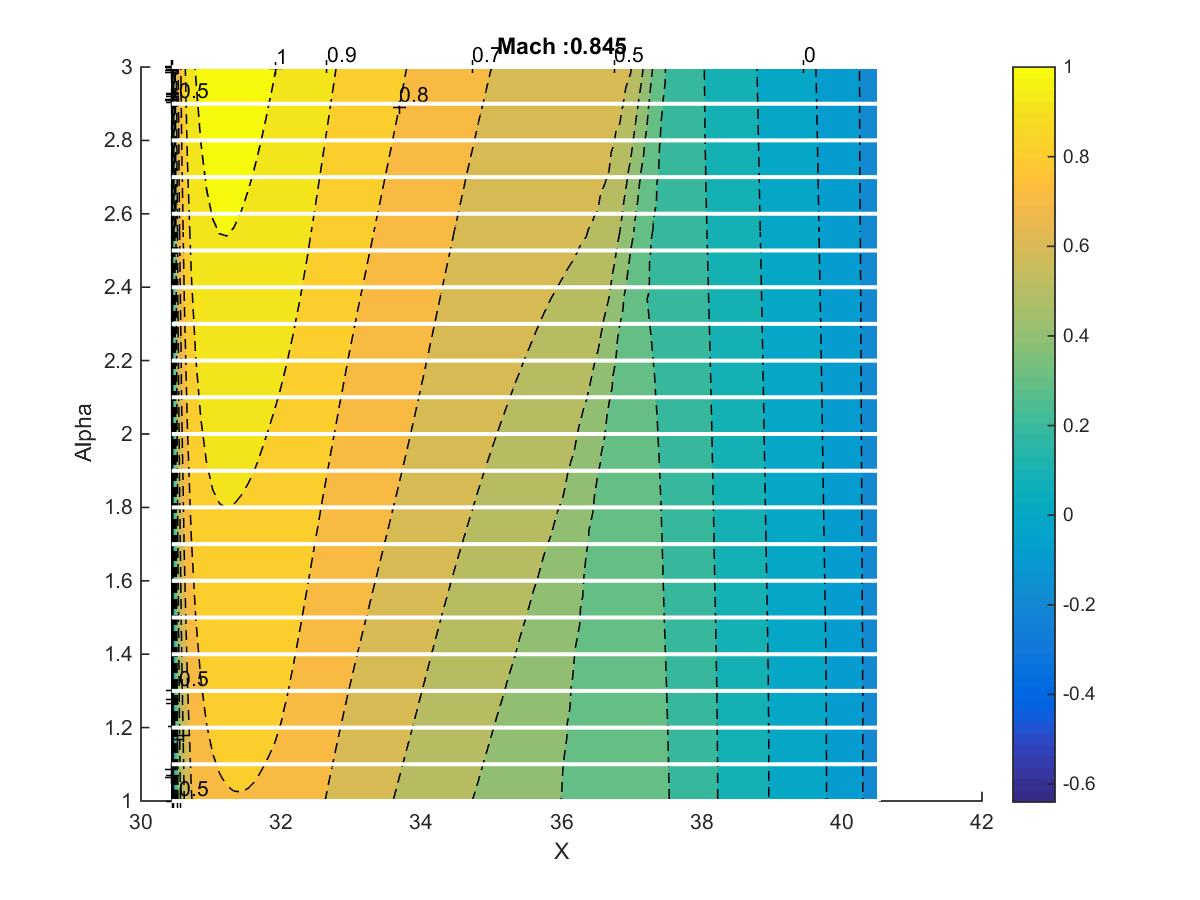
\includegraphics[width=0.45\textwidth]{images/CRM-clean-testSnapshots_cut1_MachSweepContF845}\label{subfig:alphaSweepCut1}}\quad
    \subfigure[{Interpolation performed at constant \(Mach = 0.845\) and \(\alpha = [1, 3]\) for the location \(y/b = 0.84\). The color coding denotes coefficient of pressure for upper half of airfoil, The x-axis denotes chord-wise location and y-axis denotes \(\alpha\). White lines denote presence of a pressure snapshot due to CFD run, everything in between is interpolation. Dashed black lines denote constant pressure contours color between two contours has been smoothed for clarity. We observe a single shock near \(\alpha = 3\) which slowly gets converted to a double shock pattern.}]
    {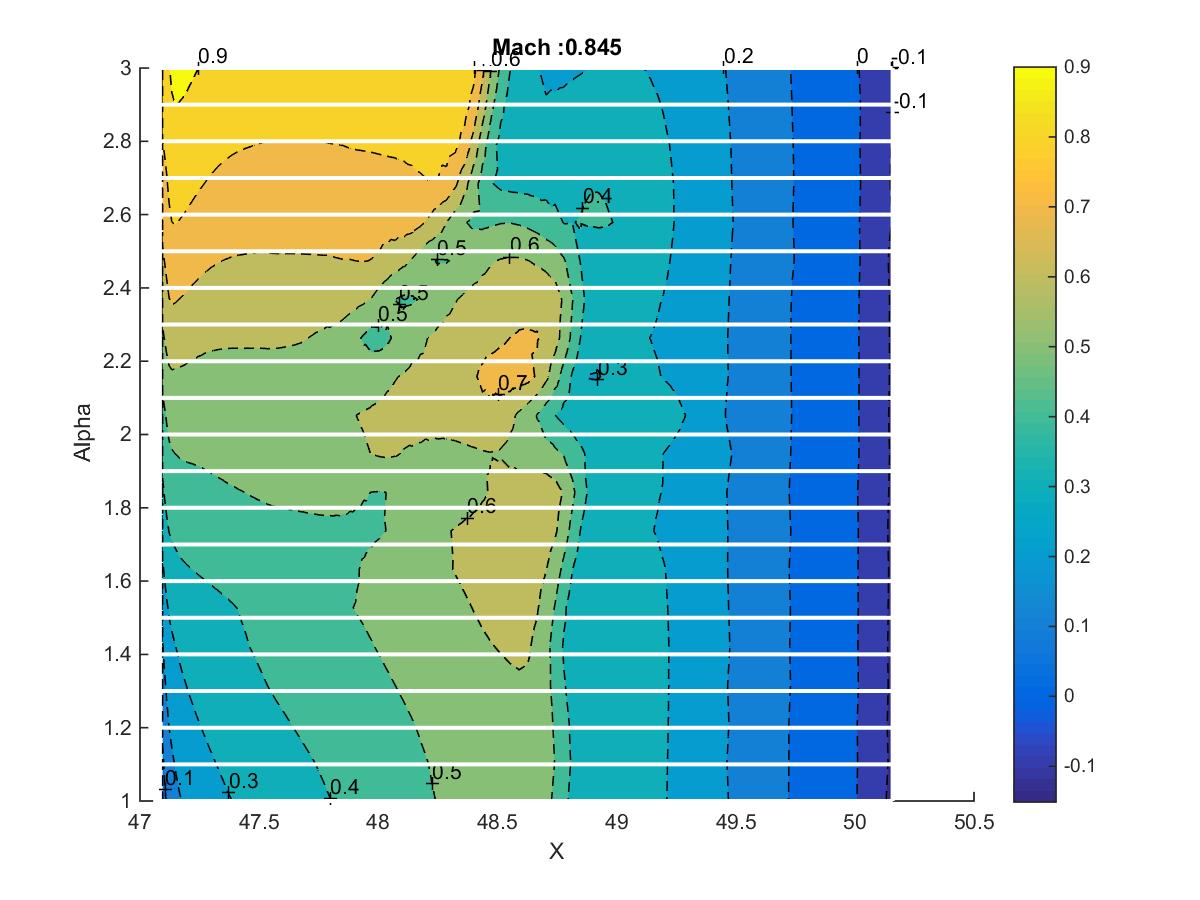
\includegraphics[width=0.45\textwidth]{images/CRM-clean-testSnapshots_cut4_MachSweepContF845}\label{subfig:alphaSweepCut4}}
  \caption{Pressure reconstructions for constant \(Mach = 0.845\) and sweeping \(\alpha \in [1, 3]\)}
\end{figure*}\label{fig:alphaSweep}

Figures \ref{subfig:alphaSweepCut1} and \ref{subfig:alphaSweepCut4} show the evaluation of pressures upon varying \(\alpha \in [1, 3]\) at locations \(y/b = 0.105\) and \(y/b = 0.84\) respectively. The color coding denotes coefficient of pressure for upper side of airfoil, The x-axis denotes chord-wise location and y-axis denotes \(\alpha\). White lines denote presence of a pressure snapshot due to CFD run, everything in between is interpolation. Dashed black lines denote constant pressure contours color between two contours has been smoothed for clarity. For figure \ref{subfig:alphaSweepCut1} we observe a strong shock near \(\alpha = 3\) which slowly gets converted to a weak shock near \(\alpha = 1\). The presence of a single shock also the reason why distributed GP performs better at this cut location. For figure \ref{subfig:alphaSweepCut4} We observe a single shock near \(\alpha = 3\) which slowly gets converted to a double shock pattern (strong first shock weak second shock). Distributed GP starts performing badly near the transition phases, this can be observed by the small pools at the transition phase from single to double shock. Notice how the pools are only formed when a CFD run is nearby, this shows that the model is not able to properly reconstruct the drop in pressure between two CFD runs. 

\subsection{Discussion}\label{subsec:ExpressingStructureKernelConclusion}
The above section shows a small sneak peek into the vast variety of kernel functions available in research papers. Due to the ability to create new kernels every problem statement comes up with an optimal structure which encodes the basic assumptions. Unfortunately finding the correct kernel is still a black art. 
 
As mentioned earlier the core aim of machine learning was to identify patterns and extrapolate on data automatically. There are two main approaches in pattern discovery; one which defines a language of kernels and iteratively adds basic kernels to come up with an explanation to the pattern in the data \cite{lloyd2014automatic}. The second is based on increasing the hypothesis space by defining a process over all stationary kernels \cite{wilson2012process}. Which approach will be retained in the long term is tough to say but research in automatic pattern detection is a highly active subject. 

It is also in the interest of this PhD to be able to extrapolate till limit-loads. Constructing a detailed kernel which can replace the parametric theoretical model is highly time-consuming. We wish to use the already constructed theoretical model as a prior into our model. How to use a parametric model for extrapolation will be discussed in the next section.


%%% Local Variables: 
%%% mode: latex
%%% TeX-master: "isae-report-template"
%%% End: 